% Documents setup
\documentclass[french,11pt]{book}

% fix for pandoc 1.14
\providecommand{\tightlist}{%
  \setlength{\itemsep}{0pt}\setlength{\parskip}{0pt}}

\usepackage{tabu} % https://tex.stackexchange.com/questions/50332/vertical-spacing-of-a-table-cell

% Location of the csas-style repository: adjust path as needed
\newcommand{\locRepo}{csas-style}

% Use the style file in the csas-style repository (res-doc.sty)
\usepackage{\locRepo/res-doc-french}

% header-includes from R markdown entry


% Headers and footers
\lhead{}
% \lhead{}
\rhead{}
% \rfoot{DRAFT - DO NOT CITE}

%%%% Commands for title page etc %%%%%

% Publication year
\newcommand{\rdYear}{2021}

% Publication month
\newcommand{\rdMonth}{}

% Report number
\newcommand{\rdNumber}{8}

% Region
\newcommand{\rdRegion}{Pacific Region}

% Title
\newcommand{\rdTitle}{Évaluation des stratégies de rétablissement possibles pour le sébaste aux yeux jaunes (\emph{Sebastes ruberrimus}) des eaux intérieures de la Colombie-Britannique}

\newcommand{\rdISBN}{Fs70-5/2021-008F-PDF}
\newcommand{\rdCatNo}{978-0-660-38699-7}

% Author names separated by commas and ', and' for the last author in the format 'M.H. Grinnell' (use \textsuperscript{n} for addresses)
\newcommand{\rdAuth}{Dana R. Haggarty\textsuperscript{1}, Quang C. Huynh\textsuperscript{2}, Robyn E. Forrest\textsuperscript{1}, Sean C. Anderson\textsuperscript{1}, Midoli J. Bresch\textsuperscript{1}, Elise A. Keppel\textsuperscript{1}}

% Author names reversed separated by commas in the format 'Grinnell, M.H.'
\newcommand{\rdAuthRev}{Haggarty, D.R., C.R. Huynh, R.E. Forrest, S.C. Anderson, M.J. Bresch, et E.A. Keppel}

% Author addresses (use \textsuperscript{n})
\newcommand{\rdAuthAddy}{\textsuperscript{1}Station biologique du Pacifique\\
Pêches et Océans Canada, 3190, chemin Hammond Bay\\
Nanaimo (Colombie-Britannique) V9T 6N7, Canada\\

\textsuperscript{2}Institut pour les océans et la pêche\\
LRAE de l'Université de la Colombie- Britannique, 2202, Main Mall\\
Vancouver (Colombie-Britannique) V6T 1Z4, Canada\\}

\newcommand{\citationOtherLanguage}{Haggarty, D.R., Huynh, Q.C., Forrest, R.E., Anderson, S.C., Bresch, M.J., Keppel, E.A. 2021. Evaluation of potential rebuilding strategies for Inside Yelloweye Rockfish (\emph{Sebastes ruberrimus}) in British Columbia. DFO Can. Sci. Advis. Sec. Res. Doc. 2021/008. vi + 141 p.}

% Name of file with abstract and resume (see \abstract and \frenchabstract for requirements)
\newcommand{\rdAbstract}{\abstract{En vertu des politiques et de la législation canadiennes, il faut Eétablir un plan de rétablissement pour les stocks de poissons qui ont été évalués comme étant inférieurs au point de référence limite (PRL) afin de les ramener au-delà du PRL. Les plans de rétablissement doivent être fondés sur des objectifs caractérisés par 1) une cible, 2) un délai souhaité pour atteindre la cible et 3) une probabilité acceptable d'atteindre la cible. Les plans de rétablissement doivent également comprendre des mesures de gestion ou des procédures de gestion, des jalons cibles et être évalués régulièrement. \vspace{1.5mm} \break Le stock de sébaste aux yeux jaunes (\emph{Sebastes ruberrimus}) des eaux intérieures est un stock sur lequel on dispose de données limitées, présent dans la zone de gestion du poisson de fond 4B (détroit de la Reine-Charlotte, détroit de Georgie et détroit de Juan de Fuca) en Colombie-Britannique. Il a été évalué comme étant inférieur au PLR en 2010, ce qui a donné lieu à la publication d'un plan de rétablissement. Il est également inscrit en vertu de la \emph{Loi sur les espèces en péril} comme espèce préoccupante. L'actuelle procédure de gestion pour assurer le rétablissement est un total autorisé des captures (TAC) annuel fixe de 15 tonnes métriques, qui n'a pas été réévalué depuis la dernière évaluation. \vspace{1.5mm} \break Ce projet vise à fournir un avis scientifique à l'appui de la réévaluation du plan de rétablissement du sébaste aux yeux jaunes des eaux intérieures. Nous appliquons un nouveau cadre d'évaluation de la stratégie de gestion (le Cadre des procédures de gestion), récemment élaboré pour le poisson de fond de la Colombie-Britannique, afin d'évaluer le rendement des autres procédures de gestion à données limitées pour ce qui est de l'atteinte des objectifs de rétablissement. Le Cadre des procédures de gestion suit six étapes de pratiques exemplaires pour évaluer la stratégie de gestion~: 1) la définition du contexte décisionnel; 2) l'établissement des objectifs et des paramètres de rendement; 3) la précision des modèles opérationnels pour représenter le système sous-jacent et calculer les paramètres de rendement; 4) la sélection des procédures de gestion possibles; 5) la réalisation de simulations en boucle fermée afin d'évaluer le rendement des procédures de gestion; 6) la présentation des résultats pour faciliter l'évaluation des compromis. \vspace{1.5mm} \break Nous avons appliqué ce cadre pour évaluer le rendement de 34 procédures de gestion à données limitées pour ce qui est de l'atteinte de l'objectif principal, qui est de ramener le stock au-dessus du PRL sur 1,5 génération avec au moins une probabilité de réussite de 95 \% {[}19 fois sur 20{]}. Nous avons également évalué le rendement des procédures de gestion en ce qui concerne deux autres paramètres de conservation, quatre objectifs de prises moyennes et un objectif de variabilité des prises. Pour tenir compte de l'incertitude liée à la dynamique de la population sous-jacente et aux sources de données, nous avons élaboré six scénarios de modèles opérationnels de rechange, qui différaient de par les hypothèses précises du modèle et des données. Ces scénarios de modèles opérationnels ont été divisés en un « ensemble de référence » (quatre modèles opérationnels) et un « ensemble de robustesse » (deux modèles opérationnels). Nous avons conditionné tous les modèles opérationnels aux données sur les prises observées, aux indices de l'abondance et aux données accessibles sur la composition selon l'âge. Nous avons utilisé la simulation en boucle fermée pour évaluer le rendement des procédures de gestion et nous avons éliminé celles qui ne satisfaisaient pas à un ensemble de critères de base, ce qui a laissé cinq procédures de gestion possibles~: des procédures de gestion à prises constantes annuelles de 10 ou 15 tonnes et trois procédures de gestion qui ajustent le TAC en fonction de la pente relative de l'indice de l'abondance dans le relevé à la palangre sur fond dur dans les eaux intérieures. \vspace{1.5mm} \break Les cinq procédures de gestion finales atteignaient l'objectif principal avec une probabilité supérieure à 0,98 (49 fois sur 50), dans les scénarios des quatre modèles opérationnels de l'ensemble de référence, surtout qu'aucun des modèles opérationnels de l'ensemble de référence n'a estimé que le stock serait inférieur au PRL en 2020. Dans les scénarios des deux modèles opérationnels de l'ensemble de robustesse, le scénario qui simulait une plus grande variabilité dans le futur relevé à la palangre sur fond dur a donné des résultats semblables à ceux des scénarios de l'ensemble de référence. Cependant, dans le scénario qui supposait un taux de mortalité naturelle plus faible pour le stock (« M faible »), toutes les procédures de gestion avaient des probabilités plus basses d'atteindre l'objectif principal, la probabilité la plus faible étant atteinte par la procédure de gestion actuelle (prises constantes de 15 tonnes). \vspace{1.5mm} \break Nous présentons un certain nombre de visualisations pour illustrer les compromis entre les objectifs de conservation et de prises pour les différentes procédures de gestion dans d'autres scénarios de modèles opérationnels. Ces visualisations présentent les compromis sous forme de tableaux et de graphiques, destinés à faciliter le processus de sélection de la procédure de gestion finale. Étant donné que toutes les procédures de gestion ont atteint l'objectif principal dans les scénarios de l'ensemble de référence, il n'y avait pas de compromis important entre les objectifs de conservation et les objectifs de prises. Parmi les deux scénarios de l'ensemble de robustesse, les compromis étaient les plus évidents dans le scénario de M faible, où la probabilité d'atteindre l'objectif principal diminuait à mesure que la probabilité de prises moyennes à court terme de 10 tonnes augmentait. \vspace{1.5mm} \break Nous discutons des incertitudes majeures, y compris l'incertitude entourant la mortalité naturelle, la sélectivité et les prises historiques, en notant que nous avons tenté d'en tenir compte en évaluant le rendement des procédures de gestion dans plusieurs modèles opérationnels. Nous soulignons les problèmes concernant les estimations de l'état actuel du stock de sébaste aux yeux jaunes des eaux intérieures et le rôle des points de référence dans le Cadre des procédures de gestion. Nous formulons des recommandations sur la fréquence des évaluations et suggérons des déclencheurs pour la réévaluation. Nous évaluons également le rendement des procédures de gestion en ce qui concerne le respect de deux autres critères d'évaluation pour le Comité sur la situation des espèces en péril au Canada.}}

%%%% End of title page commands %%%%%

% \pdfcompresslevel=5 % faster PNGs

\setcounter{section}{0}

\bibliographystyle{csas-style/res-doc}

\usepackage{amsmath}
\usepackage{bm}

% commands and environments needed by pandoc snippets
% extracted from the output of `pandoc -s`
%% Make R markdown code chunks work
\usepackage{array}
\usepackage{amssymb,amsmath}
\usepackage{color}
\usepackage{fancyvrb}
% From default template:
\newcommand{\VerbBar}{|}
\newcommand{\VERB}{\Verb[commandchars=\\\{\}]}
\DefineVerbatimEnvironment{Highlighting}{Verbatim}{commandchars=\\\{\}}
% Add ',fontsize=\small' for more characters per line
\usepackage{framed}
\definecolor{shadecolor}{RGB}{248,248,248}
\newenvironment{Shaded}{\begin{snugshade}}{\end{snugshade}}
\newcommand{\AlertTok}[1]{\textcolor[rgb]{0.94,0.16,0.16}{#1}}
\newcommand{\AnnotationTok}[1]{\textcolor[rgb]{0.56,0.35,0.01}{\textbf{\textit{#1}}}}
\newcommand{\AttributeTok}[1]{\textcolor[rgb]{0.77,0.63,0.00}{#1}}
\newcommand{\BaseNTok}[1]{\textcolor[rgb]{0.00,0.00,0.81}{#1}}
\newcommand{\BuiltInTok}[1]{#1}
\newcommand{\CharTok}[1]{\textcolor[rgb]{0.31,0.60,0.02}{#1}}
\newcommand{\CommentTok}[1]{\textcolor[rgb]{0.56,0.35,0.01}{\textit{#1}}}
\newcommand{\CommentVarTok}[1]{\textcolor[rgb]{0.56,0.35,0.01}{\textbf{\textit{#1}}}}
\newcommand{\ConstantTok}[1]{\textcolor[rgb]{0.00,0.00,0.00}{#1}}
\newcommand{\ControlFlowTok}[1]{\textcolor[rgb]{0.13,0.29,0.53}{\textbf{#1}}}
\newcommand{\DataTypeTok}[1]{\textcolor[rgb]{0.13,0.29,0.53}{#1}}
\newcommand{\DecValTok}[1]{\textcolor[rgb]{0.00,0.00,0.81}{#1}}
\newcommand{\DocumentationTok}[1]{\textcolor[rgb]{0.56,0.35,0.01}{\textbf{\textit{#1}}}}
\newcommand{\ErrorTok}[1]{\textcolor[rgb]{0.64,0.00,0.00}{\textbf{#1}}}
\newcommand{\ExtensionTok}[1]{#1}
\newcommand{\FloatTok}[1]{\textcolor[rgb]{0.00,0.00,0.81}{#1}}
\newcommand{\FunctionTok}[1]{\textcolor[rgb]{0.00,0.00,0.00}{#1}}
\newcommand{\ImportTok}[1]{#1}
\newcommand{\InformationTok}[1]{\textcolor[rgb]{0.56,0.35,0.01}{\textbf{\textit{#1}}}}
\newcommand{\KeywordTok}[1]{\textcolor[rgb]{0.13,0.29,0.53}{\textbf{#1}}}
\newcommand{\NormalTok}[1]{#1}
\newcommand{\OperatorTok}[1]{\textcolor[rgb]{0.81,0.36,0.00}{\textbf{#1}}}
\newcommand{\OtherTok}[1]{\textcolor[rgb]{0.56,0.35,0.01}{#1}}
\newcommand{\PreprocessorTok}[1]{\textcolor[rgb]{0.56,0.35,0.01}{\textit{#1}}}
\newcommand{\RegionMarkerTok}[1]{#1}
\newcommand{\SpecialCharTok}[1]{\textcolor[rgb]{0.00,0.00,0.00}{#1}}
\newcommand{\SpecialStringTok}[1]{\textcolor[rgb]{0.31,0.60,0.02}{#1}}
\newcommand{\StringTok}[1]{\textcolor[rgb]{0.31,0.60,0.02}{#1}}
\newcommand{\VariableTok}[1]{\textcolor[rgb]{0.00,0.00,0.00}{#1}}
\newcommand{\VerbatimStringTok}[1]{\textcolor[rgb]{0.31,0.60,0.02}{#1}}
\newcommand{\WarningTok}[1]{\textcolor[rgb]{0.56,0.35,0.01}{\textbf{\textit{#1}}}}

\newcommand{\lt}{\ensuremath <}
\newcommand{\gt}{\ensuremath >}

%Defines cslreferences environment
%Required by pandoc 2.8
%Copied from https://github.com/rstudio/rmarkdown/issues/1649

\DeclareGraphicsExtensions{.png,.pdf}
\begin{document}
\renewcommand{\tablename}{Tableau}
\frontmatter

\clearpage

\hypertarget{sec:introduction}{%
\section{INTRODUCTION}\label{sec:introduction}}

Ce projet vise à fournir un avis scientifique à l'appui de la révision du plan de rétablissement du stock de sébaste aux yeux jaunes (\emph{Sebastes ruberrimus}) des eaux intérieures (DFO \protect\hyperlink{ref-ifmp2018}{2018}), conformément aux directives stratégiques nationales (DFO \protect\hyperlink{ref-dfo2009}{2009}; MPO \protect\hyperlink{ref-dfo2013}{2013}). Il applique un cadre de simulation en boucle fermée (Anderson et al. \protect\hyperlink{ref-anderson2020gfmp}{2020}\protect\hyperlink{ref-anderson2020gfmp}{a}) pour évaluer le rendement des procédures de gestion de rechange en ce qui concerne les objectifs de rétablissement du stock de sébaste aux yeux jaunes des eaux intérieures.

\hypertarget{sec:introduction-motivation}{%
\subsection{MOTIVATION~: OBLIGATIONS STRATÉGIQUES ET LÉGISLATIVES}\label{sec:introduction-motivation}}

Le Cadre pour la pêche durable du Canada jette les bases de l'approche de précaution en matière de gestion des pêches au Canada (MPO \protect\hyperlink{ref-dfo2006}{2006}; DFO \protect\hyperlink{ref-dfo2009}{2009}). Le Cadre de l'approche de précaution (DFO \protect\hyperlink{ref-dfo2009}{2009}) repose sur la définition des points de référence biologiques qui définissent les cibles de la biomasse ainsi que les seuils de biomasse faible à éviter avec une probabilité élevée. L'approche exige que la mortalité par pêche soit ajustée par rapport à deux niveaux de l'état des stocks~: un point de référence supérieur du stock (RSS) et un point de référence limite (PRL) (figure~\ref{fig:pa-illustration}). Le PRL et le RSS délimitent trois zones d'état des stocks (« critique », « de prudence » et « saine »). Il faut établir un plan de rétablissement pour les stocks de poissons canadiens qui ont été évalués comme étant inférieurs au PRL, c.-à-d.~dans la zone critique (DFO \protect\hyperlink{ref-dfo2009}{2009}), afin de les ramener au-dessus du PRL (MPO \protect\hyperlink{ref-dfo2013}{2013}).


\begin{figure}[htb]

{\centering \pdftooltip{\includegraphics[width=3.8in]{C:/GitHub/yelloweye-inside/figs-french/pa-framework}}{Figure \ref{fig:pa-illustration}} 

}

\caption{Illustration du Cadre de l'approche de précaution du MPO. D'après DFO (\protect\hyperlink{ref-dfo2009}{2009}).}\label{fig:pa-illustration}
\end{figure}
En juin 2019, d'importantes modifications apportées à la \emph{Loi sur les pêches} du Canada ont légiféré de nombreux éléments clés du Cadre pour la pêche durable, qui sont enchâssés dans les dispositions sur les stocks de poissons (\href{https://laws-lois.justice.gc.ca/fra/lois/f-14/page-3.html\#h-1175547}{article 6 de la \emph{Loi sur les pêches}}. Les dispositions relatives aux stocks de poissons exigent que les principaux stocks soient gérés à des niveaux durables, en particulier à des niveaux de biomasse supérieurs au PRL. De plus, le paragraphe 6.2(1) stipule que si un grand stock de poissons a diminué en deçà de son PRL, un plan de rétablissement doit être établi pour reconstituer le stock au-dessus du PRL. Les grands stocks de poissons seront désignés en vertu d'un règlement, le premier lot de stocks devant l'être à l'automne 2020.

En vertu des directives sur l'élaboration de plans de rétablissement au Canada (MPO \protect\hyperlink{ref-dfo2013}{2013}), les plans de rétablissement doivent être fondés sur des objectifs caractérisés par~:
\begin{enumerate}
\def\labelenumi{\arabic{enumi}.}

\item
  une cible;
\item
  un délai souhaité pour atteindre la cible;
\item
  une probabilité acceptable convenue d'atteindre la cible.
\end{enumerate}
Les plans de rétablissement doivent également comprendre des mesures de gestion planifiées (les procédures de gestion), des jalons cibles et leur rendement doit faire l'objet d'examens réguliers (tous les trois ans), en plus de la surveillance et de l'évaluation annuelles. Les directives actuelles indiquent que le délai de rétablissement doit être de 1,5 à 2 fois la durée de génération de l'espèce (MPO \protect\hyperlink{ref-dfo2013}{2013}), la durée de génération étant le nombre moyen d'années entre la naissance d'un individu et la naissance de sa progéniture.

\hypertarget{sec:introduction-background}{%
\subsection{CONTEXTE}\label{sec:introduction-background}}

Le sébaste aux yeux jaunes des eaux intérieures est présent dans la zone de gestion 4B du poisson de fond en Colombie-Britannique (Figure~\ref{fig:map-4B}). Il devrait être désigné comme grand stock de poissons à l'automne 2020, date à laquelle sa gestion sera légiférée en vertu des dispositions sur les stocks de poissons. Le stock a été évalué comme étant inférieur au PLR en 2010 (Yamanaka et al. \protect\hyperlink{ref-yamanaka2011}{2011}; DFO \protect\hyperlink{ref-dfo2012}{2012}\protect\hyperlink{ref-dfo2012}{a}). De ce fait, un plan de rétablissement a été élaboré et publié à l'annexe 9 du Plan de gestion intégrée des pêches de la région du Pacifique pour le poisson de fond (DFO \protect\hyperlink{ref-ifmp2018}{2018}). Le stock de sébaste aux yeux jaunes des eaux intérieures est également inscrit en vertu de la \emph{Loi sur les espèces en péril} (LEP) comme espèce préoccupante (COSEPAC \protect\hyperlink{ref-cosewic2008}{2008}) et il est prévu que le Comité sur la situation des espèces en péril au Canada (COSEPAC) le réévaluera en 2020. Les résultats de ce projet pourraient guider la réévaluation du COSEPAC et, éventuellement, une évaluation du potentiel de rétablissement en vertu de la LEP, s'il y a lieu (voir l'annexe~\ref{app:cosewic}).


\begin{figure}[htb]

{\centering \pdftooltip{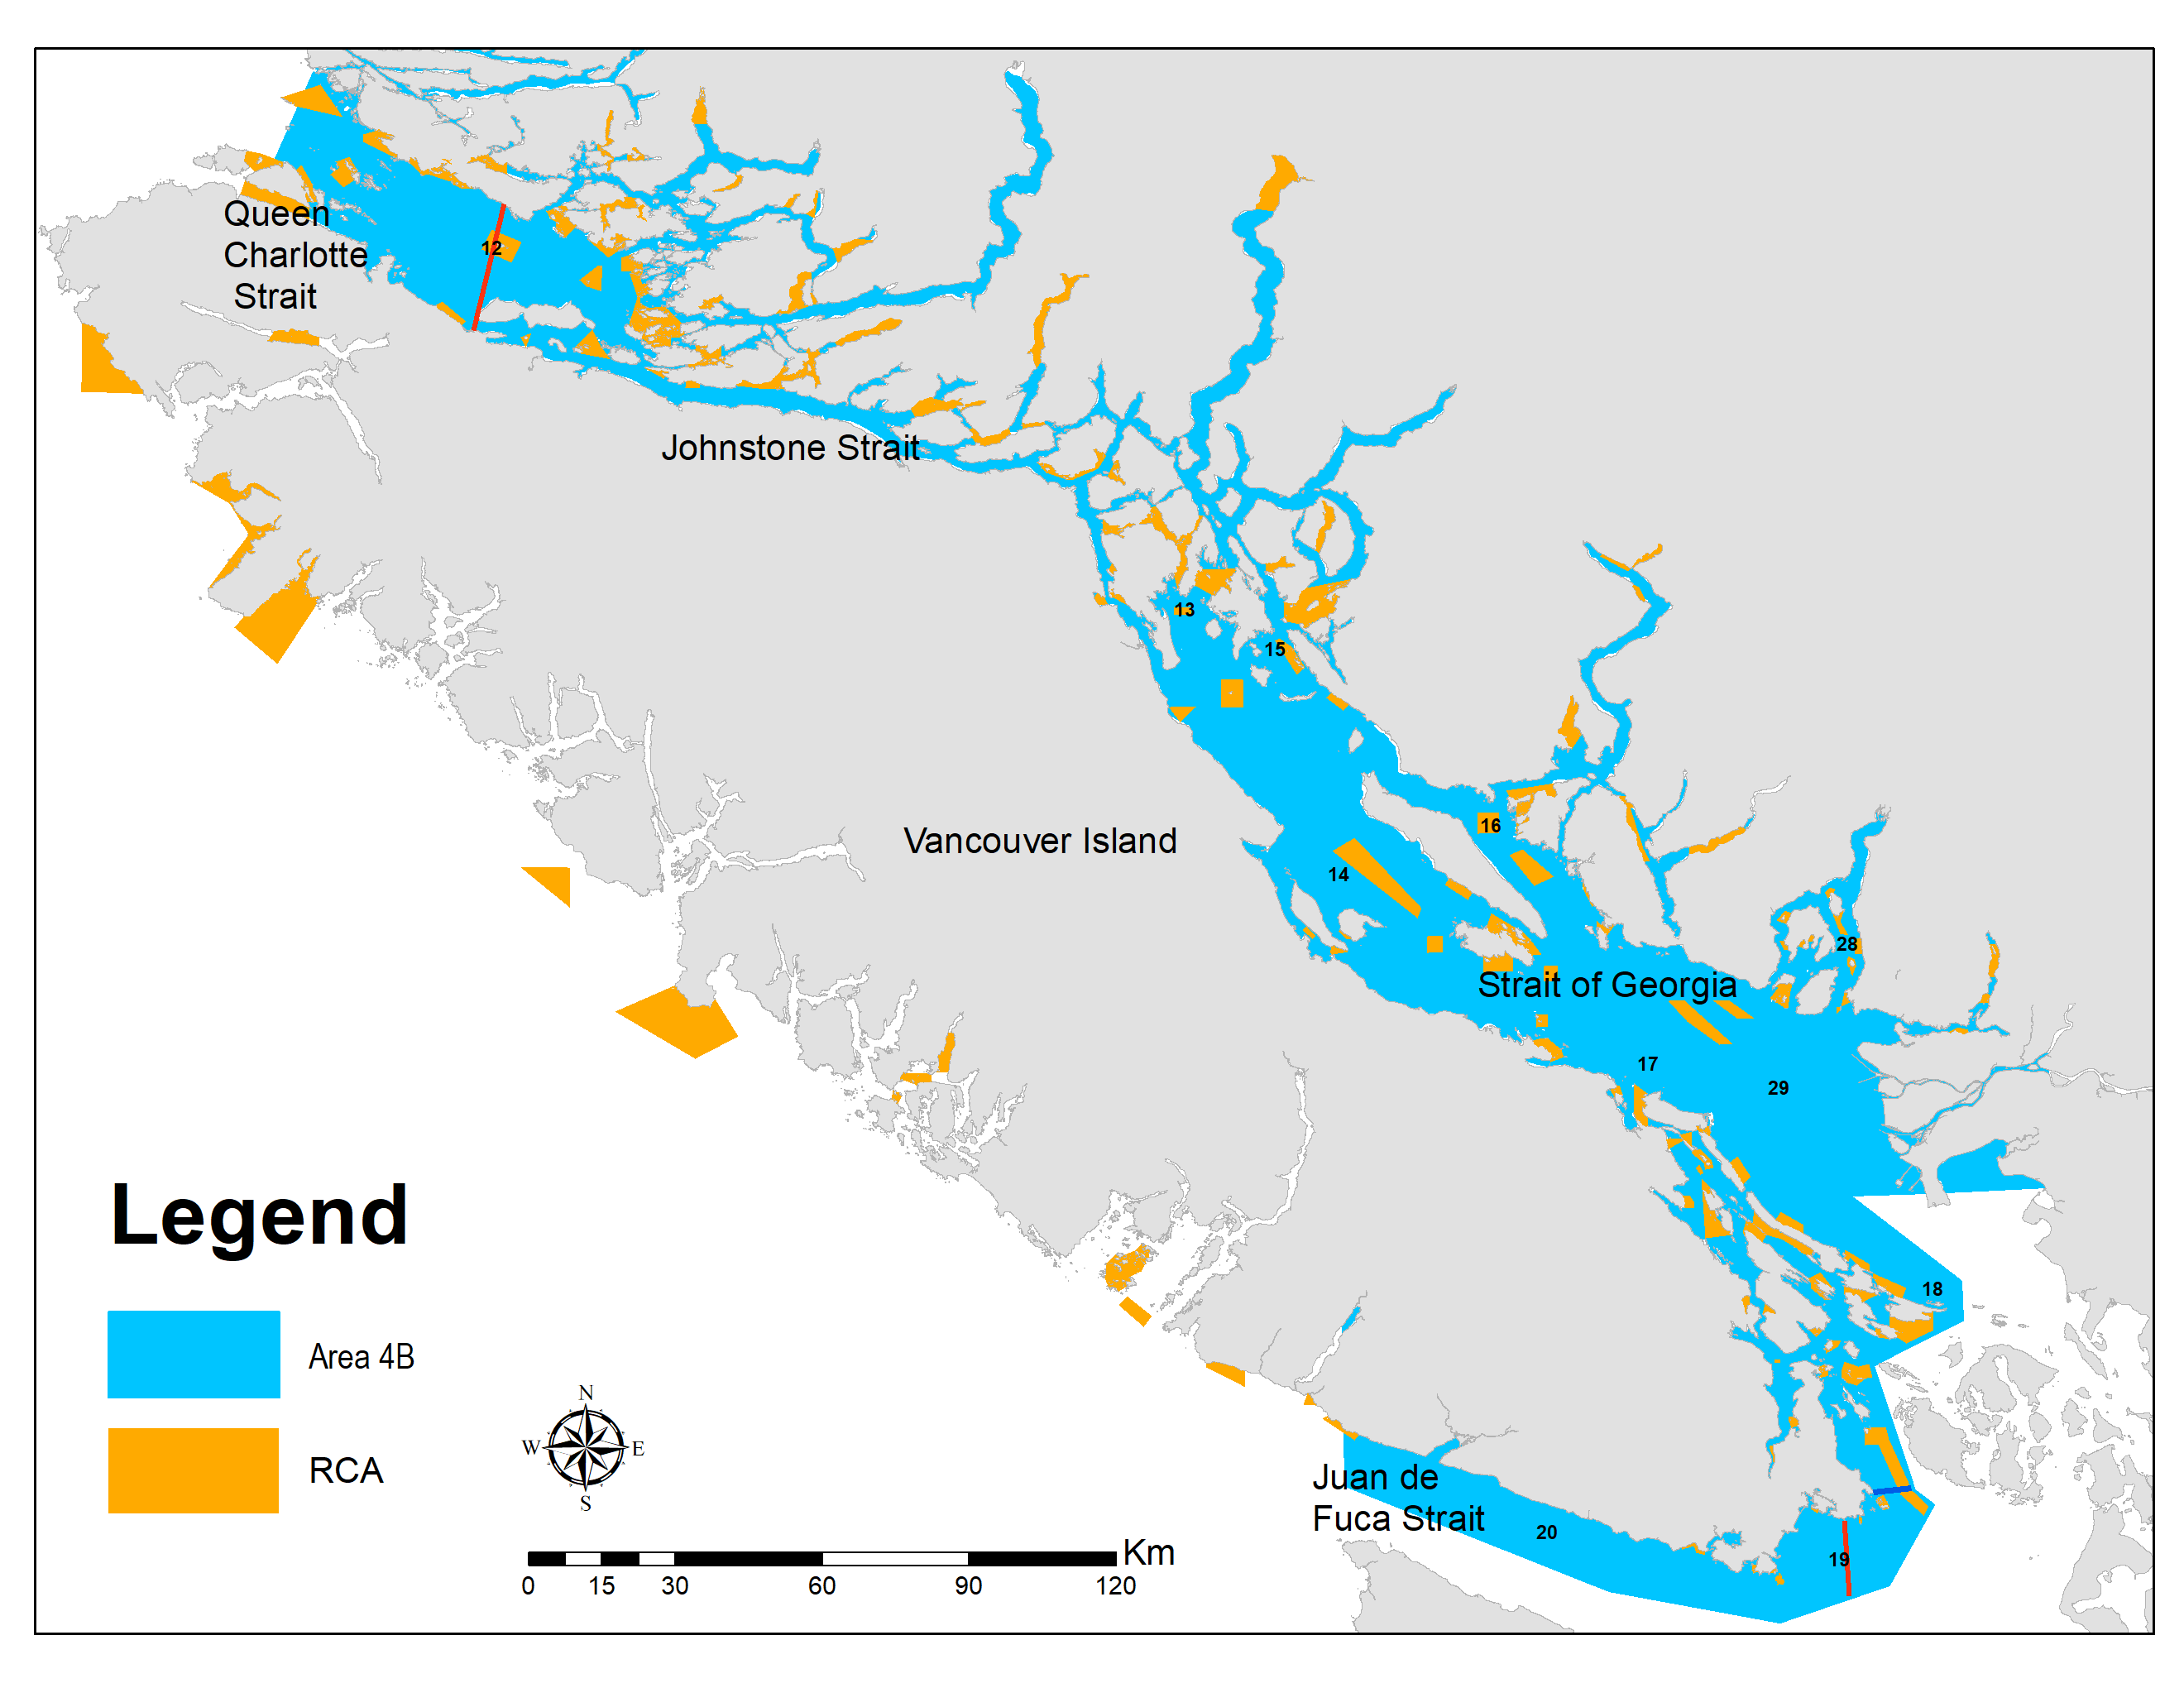
\includegraphics[width=5in]{C:/GitHub/yelloweye-inside/figs-french/InsideYE_Map_new}}{Figure \ref{fig:map-4B}} 

}

\caption{Carte de la zone de gestion 4B du poisson de fond montrant les aires de conservation du sébaste (ACS) et les limites séparant l'unité désignable (UD) du sébaste aux yeux jaunes des eaux intérieures de l'UD du sébaste aux yeux jaunes des eaux extérieures. Les lignes rouges indiquent une proposition d'ajustement de l'aire de répartition de l'UD des eaux intérieures, fondée sur des preuves génétiques récentes (Siegle \protect\hyperlink{ref-siegle2011}{2011}; Siegle et al. \protect\hyperlink{ref-siegle2013}{2013}; Andrews et al. \protect\hyperlink{ref-andrews2018}{2018}).}\label{fig:map-4B}
\end{figure}
L'objectif du plan de rétablissement actuel est de « reconstituer le stock au-dessus du PRL sur 80 ans avec une probabilité de réussite de 56 \% ». Le jalon cible est de « dégager des tendances positives au cours de chaque période de 10 ans ». La procédure de gestion actuelle du sébaste aux yeux jaunes des eaux intérieures vise à maintenir les prises annuelles totales (commerciales, récréatives, alimentaires, sociales et rituelles des Premières Nations et de relevé) à moins de 15 tonnes (voir l'annexe 9 du document DFO (\protect\hyperlink{ref-ifmp2018}{2018}) pour plus de renseignements).

D'après les directives, les plans de rétablissement au Canada doivent présenter une forte probabilité de rétablissement des stocks de poissons hors de la zone critique dans le délai prescrit (MPO \protect\hyperlink{ref-dfo2013}{2013}). Ce projet vise notamment à répondre à une préoccupation exprimée par les gestionnaires des pêches, à savoir que la probabilité de réussite de 56 \% énoncée dans le plan de rétablissement actuel (DFO \protect\hyperlink{ref-ifmp2018}{2018}) ne correspond pas à la définition d'une probabilité élevée.

Le document d'orientation indique également certaines mesures de gestion recommandées, comme le maintien des prélèvements par toutes les sources au niveau le plus bas possible, l'élaboration d'une règle de contrôle des prises et l'application de l'évaluation de la stratégie de gestion pour évaluer, par simulation, le rendement d'autres mesures de gestion pour atteindre les objectifs de rétablissement du stock (MPO \protect\hyperlink{ref-dfo2013}{2013}). Le plan de rétablissement actuel met en œuvre un total autorisé des captures annuel fixe de 15 tonnes (DFO \protect\hyperlink{ref-ifmp2018}{2018}), qui n'a pas été mis à l'essai par simulation.

Le sébaste aux yeux jaunes est une espèce qui vit longtemps (jusqu'à 121 ans en Colombie-Britannique, Keppel et Olsen \protect\hyperlink{ref-keppel2019}{2019}), dans des habitats démersaux rocheux répartis de manière irrégulière et discontinue sur la côte intérieure de la Colombie-Britannique (Yamanaka et al. \protect\hyperlink{ref-yamanaka2011}{2011}). Ces caractéristiques du cycle biologique rendent l'espèce vulnérable à la surexploitation par la pêche. Le stock des eaux intérieures est considéré comme étant à données limitées, car peu de données sont accessibles sur la composition selon l'âge, on manque de données biologiques sur les pêches commerciales, récréatives et des Premières Nations, et une incertitude entoure l'ampleur des prises historiques.

\hypertarget{sec:introduction-mse}{%
\subsection{ÉVALUATION DE LA STRATÉGIE DE GESTION}\label{sec:introduction-mse}}

À l'échelle mondiale, la fourniture d'avis scientifiques pour la gestion des pêches a évolué vers des approches axées sur l'évaluation de la stratégie de gestion (ou axées sur la gestion) (p.~ex., Butterworth et Punt \protect\hyperlink{ref-butterworth1999}{1999}; Rademeyer et al. \protect\hyperlink{ref-rademeyer2007}{2007}; Berkson et Thorson \protect\hyperlink{ref-berkson2015}{2015}; Geromont et Butterworth \protect\hyperlink{ref-geromont2015}{2015}; Carruthers et al. \protect\hyperlink{ref-carruthers2016}{2016}; Punt et al. \protect\hyperlink{ref-punt2016}{2016}). L'évaluation de la stratégie de gestion se concentre sur la détermination des procédures de gestion qui donnent les meilleurs résultats en ce qui concerne l'atteinte des objectifs convenus en matière de politique et de pêche, lorsqu'ils sont mis en œuvre dans un environnement de simulation en « boucle fermée » (figure~\ref{fig:mse-chart-basic}). Dans les pêches à production contrôlée, comme la pêche du poisson de fond en Colombie-Britannique, où les quotas sont gérés, les procédures de gestion décrivent les mesures de gestion pour l'établissement des limites des prises. Les données exigées dans les procédures de gestion peuvent varier considérablement, allant d'approches très riches en données, y compris les évaluations statistiques des prises selon l'âge avec des règles de contrôle des prises, à des règles de données simples (approches « limitées en données »), qui ne reposent que sur les données sur les prises et un indice de l'abondance (p.~ex., Geromont et Butterworth \protect\hyperlink{ref-geromont2015}{2015}; Carruthers et al. \protect\hyperlink{ref-carruthers2016}{2016}).

La simulation en boucle fermée diffère des approches d'évaluation classique des stocks parce qu'elle simule la rétroaction entre la mise en œuvre des procédures de gestion et le système sous-jacent (le stock de poisson et son environnement), décrite par un ou plusieurs modèles opérationnels. L'approche de la simulation en boucle fermée tient compte de l'effet des procédures de gestion sur le système, ainsi que des données futures recueillies dans le système et de leur utilisation chez les procédures de gestion (Punt et al. \protect\hyperlink{ref-punt2016}{2016}; Carruthers et Hordyk \protect\hyperlink{ref-carruthers2018}{2018}\protect\hyperlink{ref-carruthers2018}{a}; Anderson et al. \protect\hyperlink{ref-anderson2020gfmp}{2020}\protect\hyperlink{ref-anderson2020gfmp}{a}).


\begin{figure}[htb]

{\centering \pdftooltip{\includegraphics[width=6.3in]{C:/GitHub/yelloweye-inside/figs-french/mse-chart-simple2}}{Figure \ref{fig:mse-chart-basic}} 

}

\caption{Illustration du processus de simulation en boucle fermée des pêches d'après Anderson et al. (\protect\hyperlink{ref-anderson2020gfmp}{2020}\protect\hyperlink{ref-anderson2020gfmp}{a}), selon Punt et al. (\protect\hyperlink{ref-punt2016}{2016}). La procédure de gestion peut être fondée sur une règle de données simple (p.~ex., réduire les prises autorisées de x \% si l'indice du relevé diminue de y \%) ou peut être un modèle d'estimation combiné à une règle de contrôle des prises.}\label{fig:mse-chart-basic}
\end{figure}
\hypertarget{sec:introduction-approach}{%
\subsection{APPROCHE}\label{sec:introduction-approach}}

En raison des données limitées sur le stock de sébaste aux yeux jaunes des eaux intérieures, il est difficile d'évaluer le rendement prévu des mesures de gestion nécessaires pour rendre le stock conforme aux dispositions sur les stocks de poissons, c.-à-d.~pour le faire sortir de la zone critique dans le délai convenu et avec la probabilité convenue. La simulation-mise à l'essai en boucle fermée des procédures de gestion à données limitées permet d'évaluer le rendement relatif des procédures de gestion dans un éventail d'incertitudes entourant, par exemple, la biologie sous-jacente des poissons, l'erreur d'observation, l'erreur d'estimation et l'erreur de mise en œuvre (p.~ex., Kell et al. \protect\hyperlink{ref-kell2006}{2006}; Carruthers et al. \protect\hyperlink{ref-carruthers2016}{2016}).

Depuis 2017, une entente de partenariat entre l'Université de la Colombie-Britannique et le MPO (DFO \protect\hyperlink{ref-dfo_dlmtool_2017}{2017}) a facilité l'élaboration de deux progiciels à accès libre pour l'évaluation de la stratégie de gestion, mis en œuvre dans l'environnement de programmation statistique R (R Core Team \protect\hyperlink{ref-r2019}{2019})~: l'outil pour les méthodes à données limitées (DLMtool) (Carruthers et Hordyk \protect\hyperlink{ref-carruthers2018}{2018}\protect\hyperlink{ref-carruthers2018}{a}, \protect\hyperlink{ref-carruthers_hordyk_2018}{2018}\protect\hyperlink{ref-carruthers_hordyk_2018}{b}) et l'outil pour l'évaluation de la stratégie de gestion (MSEtool) (Huynh et al. \protect\hyperlink{ref-huynh_msetool_2019}{2019}). Après plusieurs années de développement, ces progiciels sont parmi les logiciels les plus rapides, les plus souples et les plus extensibles pour évaluer les stratégies de gestion des pêches. Ils peuvent être appliqués à des stocks pauvres ou riches en données, permettant d'évaluer rapidement plusieurs procédures de gestion en fonction d'objectifs de conservation et de pêche personnalisables, et d'évaluer les principaux compromis.

\hypertarget{sec:introduction-mp-framework}{%
\subsubsection{Cadre des procédures de gestion du poisson de fond en Colombie-Britannique}\label{sec:introduction-mp-framework}}

Le Cadre des procédures de gestion pour le poisson de fond en Colombie-Britannique (Anderson et al. \protect\hyperlink{ref-anderson2020gfmp}{2020}\protect\hyperlink{ref-anderson2020gfmp}{a}) a été élaboré parallèlement au présent document pour évaluer le rendement d'un large éventail de procédures de gestion pour les espèces de poisson de fond à données limitées. Le Cadre des procédures de gestion fait largement appel aux fonctions de DLMtool et de MSEtool, avec l'appui d'un progiciel R gfdlm (Anderson et al. \protect\hyperlink{ref-gfdlm}{2020}\protect\hyperlink{ref-gfdlm}{c}) rédigé par les auteurs de Anderson et al. (\protect\hyperlink{ref-anderson2020gfmp}{2020}\protect\hyperlink{ref-anderson2020gfmp}{a}), qui contient un ensemble d'outils de soutien logiciel et des visualisations personnalisées.

Nous suivons le Cadre des procédures de gestion pour sélectionner les procédures de gestion afin d'établir des limites des prises pour les stocks de poissons de fond à données limitées (Anderson et al. \protect\hyperlink{ref-anderson2020gfmp}{2020}\protect\hyperlink{ref-anderson2020gfmp}{a}). Notre évaluation du plan de rétablissement du sébaste aux yeux jaunes des eaux intérieures constitue la première application du Cadre des procédures de gestion pour produire un avis scientifique à l'appui des décisions sur les prises. Le cadre suit six étapes de pratiques exemplaires décrites ci-après et plus en détail dans Anderson et al. (\protect\hyperlink{ref-anderson2020gfmp}{2020}\protect\hyperlink{ref-anderson2020gfmp}{a}).

Les étapes des pratiques exemplaires sont fondées sur un examen effectué par Punt et al. (\protect\hyperlink{ref-punt2016}{2016}), qui a cerné cinq étapes clés du processus d'évaluation de la stratégie de gestion (étapes 2 à 6 ci-après). Une première étape supplémentaire du Cadre des procédures de gestion, qui définit le contexte décisionnel, a été définie par Gregory et al. (\protect\hyperlink{ref-gregory2012}{2012}) et Cox et Benson (\protect\hyperlink{ref-cox2016}{2016}). En grande partie, le logiciel DLMtool a été conçu pour permettre aux praticiens de suivre ces étapes (figure~\ref{fig:mse-chart}; Carruthers et Hordyk \protect\hyperlink{ref-carruthers2018}{2018}\protect\hyperlink{ref-carruthers2018}{a}).



Les six étapes sont les suivantes~:

Étape 1~: Définition du contexte décisionnel.

Étape 2~: Choix des objectifs et des paramètres de rendement.

Étape 3~: Choix des incertitudes/spécification des modèles opérationnels.

Étape 4~: Détermination des procédures de gestion possibles.

Étape 5~: Simulation de l'application des procédures de gestion.

Étape 6~: Présentation des résultats et choix de la procédure de gestion.

\clearpage
\begin{figure}[htb]

{\centering \pdftooltip{\includegraphics[width=\textwidth]{C:/GitHub/yelloweye-inside/figs-french/mse-chart}}{Figure \ref{fig:mse-chart}} 

}

\caption{Les étapes du processus d'évaluation de la stratégie de gestion selon Punt et al. (\protect\hyperlink{ref-punt2016}{2016}), tel que mis en œuvre dans DLMtool. Copié de Anderson et al. (\protect\hyperlink{ref-anderson2020gfmp}{2020}\protect\hyperlink{ref-anderson2020gfmp}{a}) et adapté de Carruthers et Hordyk (\protect\hyperlink{ref-carruthers2018}{2018}\protect\hyperlink{ref-carruthers2018}{a}). Cette figure complète la figure~\ref{fig:mse-chart-basic}.}\label{fig:mse-chart}
\end{figure}
Après la sélection et la mise en œuvre de la procédure de gestion pour l'établissement de la limite des prises (figure~\ref{fig:mse-chart}; par exemple, application de l'algorithme de la procédure de gestion sélectionnée à l'indice du relevé observé), la dernière étape nécessaire consiste à surveiller et à évaluer périodiquement le rendement de la procédure de gestion (MPO \protect\hyperlink{ref-dfo2013}{2013}; Dowling et al. \protect\hyperlink{ref-dowling2015a}{2015}; Carruthers et Hordyk \protect\hyperlink{ref-carruthers2018}{2018}\protect\hyperlink{ref-carruthers2018}{a}). Cela peut se faire par des moyens informels, comme à l'aide de la rétroaction des pêcheurs et des données des relevés (p.~ex., Cox et Kronlund \protect\hyperlink{ref-cox2008a}{2008}), ou au moyen de mesures statistiques plus formelles, où l'on compare les données observées aux prévisions des modèles opérationnels pour vérifier si le système fonctionne comme prévu (Butterworth \protect\hyperlink{ref-butterworth2008}{2008}; Carruthers et Hordyk \protect\hyperlink{ref-carruthers_hordyk_2018}{2018}\protect\hyperlink{ref-carruthers_hordyk_2018}{b}; discussion dans Anderson et al. \protect\hyperlink{ref-anderson2020gfmp}{2020}\protect\hyperlink{ref-anderson2020gfmp}{a}).

Dans les sections suivantes, nous décrivons notre approche pour l'élaboration d'un éventuel plan de rétablissement du sébaste aux yeux jaunes des eaux intérieures, en suivant les six étapes des pratiques exemplaires.

\section{DONNÉES SUR LES PRISES}
\label{app:catch-data}

Le sébaste aux yeux jaunes des eaux intérieures est ciblé dans les pêches commerciales à la ligne et à l'hameçon, les pêches à des fins alimentaires, sociales et rituelles (ASR) et les pêches récréatives. La gestion de la pêche du sébaste aux yeux jaunes des eaux intérieures a commencé en 1986, avec la mise en place du permis commercial de catégorie « ZN » et des limites de prises quotidiennes pour les pêcheurs récréatifs. Une chronologie des changements de gestion pour les pêches commerciales et récréatives est présentée dans les tableaux~\ref{tab:comm-mgt-changes} et~\ref{tab:rec-mgt-changes}.

\hypertarget{sec:com-catch-data}{%
\subsection{DONNÉES SUR LES PRISES COMMERCIALES}\label{sec:com-catch-data}}

Les données sur les prises de sébaste peuvent être regroupées en trois périodes~: historique (de 1918 à 1950), début de la période électronique (de 1951 à 2005) et moderne (2006 et après). Il y a deux grandes sources d'incertitude dans la période historique et le début de la période électronique pour le sébaste aux yeux jaunes des eaux intérieures. La première est que les prises de sébastes, autres que de sébaste à longue mâchoire (\emph{Sebastes alutus}), étaient déclarées de façon regroupée (autre sébaste, ORF) pendant la période historique. Pour reconstituer les prises historiques, des auteurs du MPO ont élaboré un algorithme (Haigh et Yamanaka \protect\hyperlink{ref-haigh2011}{2011}). Cet algorithme de reconstitution applique un ratio calculé à partir d'une période pour laquelle on dispose de données crédibles sur les débarquements provenant du programme de vérification à quai des pêches à la ligne et à l'hameçon (1997--2005) pour générer une série chronologique des prises par espèce, année, secteur de pêche et zone de gestion (Haigh et Yamanaka \protect\hyperlink{ref-haigh2011}{2011}). Les données « crédibles » sur les débarquements sont tirées des années de référence où la connaissance des prises était considérée comme étant de grande qualité et stable, depuis 1997, avec le début de la présence d'observateurs à bord des chalutiers et le système de quotas individuels des bateaux (Haigh et Yamanaka \protect\hyperlink{ref-haigh2011}{2011}).

La deuxième grande source d'incertitude est l'ampleur des prises non déclarées qui étaient remises à l'eau ou rejetées en mer avant la mise en place du niveau de présence des observateurs de 100 \% en 2006. La reconstitution des prises de Haigh et Yamanaka (\protect\hyperlink{ref-haigh2011}{2011}) suppose qu'il n'y avait pas de rejet avant 1986, année où le permis ZN a été institué. On suppose qu'auparavant, tous les sébastes étaient conservés. Les rejets sont présumés être entièrement déclarés dans les bases de données du MPO depuis 2006 et le niveau de présence des observateurs en mer de 100 \%. Les prises de sébaste aux yeux jaunes non conservées (remises à l'eau ou rejetées) ont été estimées pour chaque pêche à l'aide du ratio des rejets de sébaste aux yeux jaunes par les cibles de débarquement propres à la pêche d'après les données de 2000 à 2004 des registres des observateurs des pêches à la ligne et à l'hameçon. Les prises historiques non déclarées ont ensuite été intégrées à la reconstitution des prises, pour donner un total annuel final.

La série chronologique des prises commerciales utilisée dans cette analyse (figure~\ref{fig:commcatch2} et tableau~\ref{tab:commcatch}) diffère de celle précédemment présentée en 2009 pour plusieurs raisons. Le contrôle continu de la qualité et les mises à jour de la base de données sur les prises de poisson de fond ont entraîné des différences mineures dans les données au fil du temps (Maria Surry, MPO, Station biologique du Pacifique, comm. pers., 9 mars 2020). De plus, une version antérieure de l'algorithme de reconstitution des prises a été utilisée pour élaborer la série chronologique pour l'évaluation des stocks précédente, car la version finale n'avait pas encore été publiée. D'autres améliorations apportées à l'algorithme de reconstitution ont provoqué des changements importants des prises historiques estimées certaines années (Norm Olsen, MPO, Station biologique du Pacifique, comm. pers., 9 mars 2020).

L'algorithme de reconstitution aurait pu être appliqué à toutes les années de la série chronologique jusqu'en 2005 (après quoi la vérification complète en mer et à quai est entrée en vigueur). Toutefois, pour cette analyse, nous avons utilisé les données reconstituées sur les prises de 1918 à 1985 et nous sommes passés aux données sur les prises nominales en 1986. Les prises nominales de 1986 à 2005 ont ensuite été doublées, conformément à l'évaluation précédente (Yamanaka et al. \protect\hyperlink{ref-yamanaka2011}{2011}). Nous avons choisi de doubler les prises nominales plutôt que les prises reconstituées parce que, avant l'évaluation précédente, les représentants de l'industrie nous avaient dit qu'ils n'avaient pas confiance dans la reconstitution des prises entre 1986 et 2005 et que l'échelle des prises non déclarées était probablement égale aux prises débarquées (DFO \protect\hyperlink{ref-dfo2012b}{2012}\protect\hyperlink{ref-dfo2012b}{b}). Ces indications nous ont amenés à doubler les prises pour ces années (Yamanaka et al. \protect\hyperlink{ref-yamanaka2011}{2011}). Cependant, comme les rejets sont estimés dans le cadre de l'algorithme de reconstitution des prises, dans l'analyse actuelle, nous avons doublé les prises nominales pour la période 1986--2005 (plutôt que les prises reconstituées) afin d'éviter de compter les rejets deux fois. Pour vérifier la sensibilité, nous explorons un scénario de modèle opérationnel où les prises commerciales de 1986 à 2005 n'ont pas été doublées (le scénario « Prises faibles » (2), section~\ref{sec:approach3-reference2}).
\begin{figure}[htb]

{\centering \pdftooltip{\includegraphics[width=0.8\textwidth]{knitr-figs-pdf/commcatch2-1}}{Figure \ref{fig:commcatch2}} 

}

\caption{Prises commerciales par secteur pour le sébaste aux yeux jaunes des eaux intérieures. Cette figure comprend les estimations reconstituées (1918--1985) et nominales (1986--2019) des prises en tonnes. A=Sébaste à la ligne et à l’hameçon, B=Aiguillat commun, Morue-lingue, C=Flétan, D=Chalut.}\label{fig:commcatch2}
\end{figure}
\clearpage
\begin{longtable}[t]{>{\raggedleft\arraybackslash}p{1.0cm}>{\raggedleft\arraybackslash}p{2cm}>{\raggedleft\arraybackslash}p{2cm}>{\raggedleft\arraybackslash}p{2cm}>{\raggedleft\arraybackslash}p{2cm}>{\raggedleft\arraybackslash}p{2cm}}
\caption{\label{tab:commcatch}Prises commerciales par secteur pour le sébaste aux yeux jaunes des eaux intérieures. Le tableau présente les estimations des prises reconstituées (1918--1985) et nominales (1986--2019), en tonnes. Bien que les prises nominales soient indiquées, les prises totales pour chaque année entre 1986 et 2005 ont été doublées dans tous les modèles opérationnels, sauf dans le scénario « Prises faibles », dans un souci de cohérence avec l’évaluation précédente du stock en 2012.}\\
\toprule
\textbf{Année} & \textbf{Chalut} & \textbf{Flétan} & \textbf{Aiguillat commun et morue-lingue} & \textbf{Sébaste à la ligne et à l’hameçon} & \textbf{Total}\\
\midrule
\endfirsthead
\caption*{}\\
\toprule
\textbf{Année} & \textbf{Chalut} & \textbf{Flétan} & \textbf{Aiguillat commun et morue-lingue} & \textbf{Sébaste à la ligne et à l’hameçon} & \textbf{Total}\\
\midrule
\endhead
\
\endfoot
\bottomrule
\endlastfoot
1918 & 0,00 & 3,40 & 4,90 & 8,80 & 17,10\\
1919 & 0,00 & 8,50 & 12,00 & 22,00 & 42,50\\
1920 & 0,00 & 4,30 & 6,00 & 11,00 & 21,30\\
1921 & 0,00 & 3,70 & 5,20 & 9,50 & 18,40\\
1922 & 0,00 & 4,60 & 6,50 & 12,00 & 23,10\\
1923 & 0,00 & 4,50 & 6,30 & 11,00 & 21,80\\
1924 & 0,00 & 5,10 & 7,20 & 13,00 & 25,30\\
1925 & 0,00 & 4,40 & 6,20 & 11,00 & 21,60\\
1926 & 0,00 & 5,00 & 7,10 & 13,00 & 25,10\\
1927 & 0,00 & 5,00 & 7,10 & 13,00 & 25,10\\
1928 & 0,00 & 5,10 & 7,30 & 13,00 & 25,40\\
1929 & 0,00 & 6,70 & 9,50 & 17,00 & 33,20\\
1930 & 0,00 & 6,00 & 8,60 & 16,00 & 30,60\\
1931 & 0,00 & 4,00 & 5,60 & 10,00 & 19,60\\
1932 & 0,00 & 4,50 & 6,40 & 12,00 & 22,90\\
1933 & 0,00 & 2,20 & 3,10 & 5,70 & 11,00\\
1934 & 0,00 & 2,60 & 3,70 & 6,70 & 13,00\\
1935 & 0,00 & 3,30 & 4,70 & 8,60 & 16,60\\
1936 & 0,00 & 3,60 & 5,10 & 9,30 & 18,00\\
1937 & 0,00 & 2,80 & 4,00 & 7,30 & 14,10\\
1938 & 0,00 & 10,00 & 14,00 & 25,00 & 49,00\\
1939 & 0,00 & 1,90 & 2,70 & 4,80 & 9,40\\
1940 & 0,00 & 2,00 & 2,90 & 5,30 & 10,20\\
1941 & 0,00 & 1,30 & 1,80 & 3,20 & 6,30\\
1942 & 0,00 & 2,90 & 4,10 & 7,50 & 14,50\\
1943 & 0,00 & 17,00 & 24,00 & 43,00 & 84,00\\
1944 & 0,00 & 25,00 & 36,00 & 64,00 & 125,00\\
1945 & 0,00 & 27,00 & 38,00 & 69,00 & 134,00\\
1946 & 0,00 & 18,00 & 26,00 & 46,00 & 90,00\\
1947 & 0,00 & 5,80 & 8,10 & 15,00 & 28,90\\
1948 & 0,00 & 8,80 & 12,00 & 23,00 & 43,80\\
1949 & 0,00 & 12,00 & 17,00 & 30,00 & 59,00\\
1950 & 0,00 & 5,00 & 7,00 & 13,00 & 25,00\\
1951 & 0,00 & 3,60 & 5,10 & 9,30 & 18,00\\
1952 & 0,00 & 2,80 & 3,90 & 7,10 & 13,80\\
1953 & 0,00 & 5,80 & 8,30 & 15,00 & 29,10\\
1954 & 0,00 & 3,60 & 5,10 & 9,30 & 18,00\\
1955 & 0,00 & 3,60 & 5,10 & 9,20 & 17,90\\
1956 & 0,00 & 3,40 & 4,80 & 8,80 & 17,00\\
1957 & 0,00 & 5,90 & 8,40 & 15,00 & 29,30\\
1958 & 0,00 & 8,60 & 12,00 & 22,00 & 42,60\\
1959 & 0,00 & 8,80 & 13,00 & 23,00 & 44,80\\
1960 & 0,00 & 7,20 & 10,00 & 18,00 & 35,20\\
1961 & 0,00 & 5,30 & 7,60 & 14,00 & 26,90\\
1962 & 0,00 & 8,60 & 12,00 & 22,00 & 42,60\\
1963 & 0,00 & 6,60 & 9,30 & 17,00 & 32,90\\
1964 & 0,00 & 4,00 & 5,60 & 10,00 & 19,60\\
1965 & 0,00 & 3,60 & 5,10 & 9,20 & 17,90\\
1966 & 0,00 & 2,90 & 4,10 & 7,40 & 14,40\\
1967 & 0,00 & 4,50 & 6,30 & 11,00 & 21,80\\
1968 & 0,00 & 4,80 & 6,80 & 12,00 & 23,60\\
1969 & 0,00 & 5,60 & 7,90 & 14,00 & 27,50\\
1970 & 0,00 & 6,80 & 10,00 & 18,00 & 34,80\\
1971 & 0,00 & 5,80 & 8,30 & 15,00 & 29,10\\
1972 & 0,00 & 6,50 & 9,10 & 17,00 & 32,60\\
1973 & 0,00 & 7,90 & 11,00 & 20,00 & 38,90\\
1974 & 0,00 & 3,90 & 5,50 & 10,00 & 19,40\\
1975 & 0,00 & 3,10 & 4,40 & 8,00 & 15,50\\
1976 & 0,00 & 3,80 & 5,40 & 10,00 & 19,20\\
1977 & 0,10 & 11,00 & 15,00 & 27,00 & 53,10\\
1978 & 0,20 & 12,00 & 17,00 & 31,00 & 60,20\\
1979 & 0,00 & 19,00 & 27,00 & 49,00 & 95,00\\
1980 & 0,00 & 14,00 & 20,00 & 36,00 & 70,00\\
1981 & 0,00 & 16,00 & 23,00 & 42,00 & 81,00\\
1982 & 5,90 & 22,00 & 14,00 & 13,00 & 54,90\\
1983 & 7,90 & 23,00 & 14,00 & 6,60 & 51,50\\
1984 & 30,00 & 27,00 & 8,40 & 9,40 & 74,80\\
1985 & 68,00 & 34,00 & 7,60 & 10,00 & 119,60\\
1969 & 0,04 & 0,00 & 0,00 & 0,00 & 0,04\\
1977 & 0,10 & 0,00 & 0,00 & 0,00 & 0,10\\
1978 & 0,18 & 0,00 & 0,00 & 0,00 & 0,18\\
1979 & 0,02 & 0,00 & 0,00 & 0,00 & 0,02\\
1980 & 0,00 & 0,00 & 0,00 & 0,00 & 0,00\\
1983 & 0,03 & 0,00 & 0,00 & 0,00 & 0,03\\
1984 & 0,00 & 0,00 & 0,00 & 0,00 & 0,00\\
1986 & 0,00 & 0,00 & 0,00 & 157,89 & 157,89\\
1987 & 0,35 & 0,00 & 0,00 & 97,73 & 98,08\\
1988 & 0,01 & 0,00 & 0,00 & 128,31 & 128,32\\
1989 & 0,01 & 0,00 & 0,00 & 119,42 & 119,43\\
1990 & 0,00 & 0,00 & 0,00 & 128,53 & 128,53\\
1991 & 0,00 & 0,00 & 0,00 & 60,63 & 60,63\\
1992 & 0,00 & 0,00 & 0,00 & 25,55 & 25,55\\
1993 & 0,01 & 0,00 & 0,00 & 41,59 & 41,60\\
1994 & 0,36 & 0,00 & 0,00 & 88,81 & 89,17\\
1995 & 0,05 & 0,65 & 0,00 & 34,24 & 34,94\\
1996 & 0,04 & 1,27 & 0,06 & 25,22 & 26,59\\
1997 & 0,00 & 2,44 & 0,05 & 23,09 & 25,58\\
1998 & 0,01 & 6,34 & 0,23 & 29,04 & 35,62\\
1999 & 0,00 & 1,57 & 0,07 & 23,04 & 24,68\\
2000 & 0,00 & 0,44 & 0,00 & 26,79 & 27,23\\
2001 & 0,01 & 0,83 & 0,21 & 23,23 & 24,28\\
2002 & 0,00 & 0,02 & 0,03 & 3,32 & 3,37\\
2003 & 0,01 & 0,00 & 1,48 & 3,51 & 5,00\\
2004 & 0,00 & 0,19 & 1,77 & 2,08 & 4,04\\
2005 & 0,00 & 0,02 & 3,45 & 2,23 & 5,70\\
2006 & 0,00 & 0,49 & 2,22 & 1,06 & 3,77\\
2007 & 0,01 & 1,74 & 2,43 & 3,34 & 7,52\\
2008 & 0,00 & 2,26 & 2,80 & 4,40 & 9,46\\
2009 & 0,00 & 0,93 & 2,85 & 2,67 & 6,45\\
2010 & 0,00 & 1,12 & 2,56 & 2,84 & 6,52\\
2011 & 0,00 & 1,26 & 1,48 & 4,00 & 6,74\\
2012 & 0,00 & 1,23 & 1,26 & 2,61 & 5,10\\
2013 & 0,00 & 0,28 & 1,34 & 3,51 & 5,13\\
2014 & 0,00 & 1,03 & 0,55 & 3,48 & 5,06\\
2015 & 0,00 & 0,19 & 1,80 & 3,51 & 5,50\\
2016 & 0,04 & 0,49 & 0,62 & 3,18 & 4,33\\
2017 & 0,01 & 1,26 & 0,00 & 5,75 & 7,02\\
2018 & 0,02 & 0,29 & 0,00 & 2,42 & 2,73\\
2019 & 0,00 & 0,07 & 0,01 & 2,71 & 2,79\\
2020 & 0,01 & 0,00 & 0,00 & 0,32 & 0,33\\*
\end{longtable}
\clearpage

\hypertarget{sec:rec-catch-data}{%
\subsection{DONNÉES SUR LES PRISES RÉCRÉATIVES}\label{sec:rec-catch-data}}

En 2012, le MPO a établi un relevé sur Internet destiné aux détenteurs de permis de pêche en eaux de marées à l'échelle de la côte (iRec) qui permet de recueillir des données sur le sébaste aux yeux jaunes (MPO \protect\hyperlink{ref-dfo2015}{2015}). Toutefois, on n'a pas étalonné les résultats de ce relevé pour tenir compte des incertitudes comme le biais de non-réponse. C'est pourquoi les données iRec n'ont pas été incluses dans cette analyse.

\hypertarget{sec:recon-rec-catch-data}{%
\subsubsection{Prises récréatives historiques reconstituées}\label{sec:recon-rec-catch-data}}

Les prises récréatives historiques, avant 1982, ont été reconstituées pour l'évaluation précédente d'après les tendances de l'effort de pêche dégagées d'entrevues avec les propriétaires d'un camp de pêche récréative (Yamanaka et al. \protect\hyperlink{ref-yamanaka2011}{2011}). Nous avons utilisé la même série chronologique des prises récréatives reconstituées pour l'analyse actuelle (tableau~\ref{tab:rectable}).

\hypertarget{sec:creel-catch-data}{%
\subsubsection{Données des relevés par interrogation de pêcheurs, de 1982 à 2019}\label{sec:creel-catch-data}}

Les prises annuelles de sébaste aux yeux jaunes des eaux intérieures dans la pêche récréative sont estimées par les relevés par interrogation de pêcheurs dans le détroit de Georgie (DG) et du nord de l'île de Vancouver (NIV) dans tous les SGPP (figure~\ref{fig:map-4B}). Les relevés portent sur les SGPP 12--20, 28 et 29 (Zetterberg et Carter \protect\hyperlink{ref-zetterberg2010}{2010}). Les prises de sébaste ont été enregistrées dans les secteurs 13--19, 28 et 29 depuis 1982, mais n'étaient pas dénombrées par espèce avant 2000. Dans le SGPP 12, les sébastes sont dénombrés par espèce depuis 2000, sans enregistrement avant 2000 (Zetterberg et Carter \protect\hyperlink{ref-zetterberg2010}{2010}).

Nous avons suivi la même méthode que celle de Yamanaka et al. (\protect\hyperlink{ref-yamanaka2011}{2011}) pour estimer les prises récréatives de sébaste aux yeux jaunes des eaux intérieures de 1982 à 1999. Tout d'abord, pour tous les SGPP autres que le SGPP 12, nous avons calculé la proportion moyenne des prises de sébaste aux yeux jaunes par rapport aux prises totales de sébaste pour chaque SGPP en 2000 et en 2001. Nous avons ensuite utilisé les proportions moyennes pour dériver les estimations des prises de sébaste aux yeux jaunes des prises totales de sébastes par SGPP de 1982 à 1999. L'évaluation précédente supposait que la proportion des prises de sébaste aux yeux jaunes dans le SGPP 12, sur le total des prises de sébaste aux yeux jaunes dans le détroit de Georgie, demeurerait relativement constante dans le temps. Par conséquent, pour estimer les prises de sébaste aux yeux jaunes dans le SGPP 12 pour les années 1982--1999, nous avons calculé la proportion de sébastes aux yeux jaunes capturés dans le SGPP 12, sur le total de sébastes aux yeux jaunes capturés dans le détroit de Georgie en 2000 et en 2001. Nous avons ensuite multiplié la proportion moyenne pour 2000 et 2001 par le total des prises de sébaste aux yeux jaunes estimées pour le reste du détroit de Georgie (somme des secteurs 13--19, 28 et 29) afin d'estimer les prises de sébaste aux yeux jaunes dans le SGPP 12 par année (tableau~\ref{tab:recbyarea}). Pour assurer la conformité à l'évaluation précédente, nous avons appliqué un ajustement de 1,09 à l'effort annuel total pour tenir compte du manque d'enregistrements dans le SGPP 12, où l'effort n'a pas été enregistré avant 2000. Nous avons converti les nombres de sébastes en poids en multipliant par 2,49 kg le poids moyen de l'échantillon de sébaste aux yeux jaunes prélevé dans les relevés par interrogation de pêcheurs entre 2000 et 2008.

Nous n'avons pas élaboré d'indice des CPUE pour la pêche récréative, bien que des données récentes sur les relevés par interrogation de pêcheurs soient accessibles. Depuis l'imposition de procédures de gestion visant la conservation des sébastes (tableau~\ref{tab:rec-mgt-changes}), une tendance à l'évitement actif du sébaste a été observée dans les pêches récréatives. De ce fait, nous craignons qu'une série de CPUE pour la pêche récréative ne tienne pas compte des changements de l'abondance et ne soit donc trompeuse aux fins de l'évaluation.
\begin{figure}[htb]

{\centering \pdftooltip{\includegraphics[width=0.8\textwidth]{knitr-figs-pdf/reccatch-1}}{Figure \ref{fig:reccatch}} 

}

\caption{Prises récréatives de sébaste aux yeux jaunes des eaux intérieures. La ligne noire indique les prises reconstituées et les barres sont les données des relevés par interrogation de pêcheurs. Les données sont une combinaison des prises reconstituées (1918--1981), des prises analysées à partir du total des prises de sébaste dans les relevés par interrogation de pêcheurs (1982--1999) et des prises provenant de relevés sur certaines espèces par interrogation de pêcheurs (1982--2019).}\label{fig:reccatch}
\end{figure}
\begin{longtable}[t]{ccc}
\caption{\label{tab:rectable}Prises récréatives de sébaste aux yeux jaunes des eaux intérieures. Les données sont une combinaison des prises reconstituées (1918--1981), des prises analysées à partir du total des prises de sébaste dans les relevés par interrogation de pêcheurs (1982--1999) et des prises provenant de relevés sur certaines espèces par interrogation de pêcheurs (1982--2019).}\\
\toprule
\textbf{Année} & \textbf{Prises (t)} & \textbf{Effort (sorties de bateaux)}\\
\midrule
\endfirsthead
\caption*{}\\
\toprule
\textbf{Année} & \textbf{Prises (t)} & \textbf{Effort (sorties de bateaux)}\\
\midrule
\endhead
\
\endfoot
\bottomrule
\endlastfoot
1918 & 0,9 & 16600\\
1919 & 0,9 & 16600\\
1920 & 0,9 & 16600\\
1921 & 0,9 & 16600\\
1922 & 0,9 & 16600\\
1923 & 0,9 & 16600\\
1924 & 0,9 & 16600\\
1925 & 0,9 & 16600\\
1926 & 0,9 & 16600\\
1927 & 0,9 & 16600\\
1928 & 0,9 & 16600\\
1929 & 0,9 & 16600\\
1930 & 0,9 & 16600\\
1931 & 0,9 & 16600\\
1932 & 0,9 & 16600\\
1933 & 0,9 & 16600\\
1934 & 0,9 & 16600\\
1935 & 0,9 & 16600\\
1936 & 0,9 & 16600\\
1937 & 0,9 & 16600\\
1938 & 0,9 & 16600\\
1939 & 0,9 & 16600\\
1940 & 0,9 & 16600\\
1941 & 0,9 & 16600\\
1942 & 0,9 & 16600\\
1943 & 0,9 & 16600\\
1944 & 0,9 & 16600\\
1945 & 0,9 & 16600\\
1946 & 1 & 19800\\
1947 & 2 & 39500\\
1948 & 3,1 & 59300\\
1949 & 4,1 & 79000\\
1950 & 5,1 & 98800\\
1951 & 6,1 & 118600\\
1952 & 7,2 & 138300\\
1953 & 8,2 & 158100\\
1954 & 9,2 & 177800\\
1955 & 10,2 & 197600\\
1956 & 11,3 & 217400\\
1957 & 12,3 & 237100\\
1958 & 13,3 & 256900\\
1959 & 14,3 & 276600\\
1960 & 15,4 & 296400\\
1961 & 17,2 & 332800\\
1962 & 17,2 & 332800\\
1963 & 17,2 & 332800\\
1964 & 17,2 & 332800\\
1965 & 17,2 & 332800\\
1966 & 17,2 & 332800\\
1967 & 17,2 & 332800\\
1968 & 17,2 & 332800\\
1969 & 17,2 & 332800\\
1970 & 18,2 & 350300\\
1971 & 19,1 & 367800\\
1972 & 20 & 385300\\
1973 & 20,9 & 402900\\
1974 & 21,8 & 420400\\
1975 & 22,7 & 437900\\
1976 & 23,6 & 455400\\
1977 & 24,5 & 472900\\
1978 & 25,4 & 490400\\
1979 & 26,3 & 507900\\
1980 & 27,2 & 525500\\
1981 & 15,9 & 306500\\
1982 & 33,4 & 609738\\
1983 & 29,5 & 581764\\
1984 & 22 & 709686\\
1985 & 24,8 & 685082\\
1986 & 32,1 & 635438\\
1987 & 21,6 & 642698\\
1988 & 32,9 & 714448\\
1989 & 36,2 & 657638\\
1990 & 29,3 & 572527\\
1991 & 33,3 & 493093\\
1992 & 26,3 & 500668\\
1993 & 17 & 542848\\
1994 & 26,6 & 480411\\
1995 & 21,2 & 352770\\
1996 & 19,8 & 314722\\
1997 & 15,6 & 297399\\
1998 & 14,3 & 181874\\
1999 & 11,4 & 178133\\
2000 & 16 & 201870\\
2001 & 22 & 206345\\
2002 & 8,4 & 217408\\
2003 & 9,5 & 197227\\
2004 & 7,7 & 148898\\
2005 & 3,9 & 125019\\
2006 & 6,2 & 119256\\
2007 & 2,4 & 128332\\
2008 & 4,4 & 110568\\
2009 & 4,1 & 119343\\
2010 & 4,6 & 111307\\
2011 & 4,8 & 113544\\
2012 & 5,1 & --\\
2013 & 11,1 & 164466\\
2014 & 1,9 & 132320\\
2015 & 6,1 & 159424\\
2016 & 8,9 & 143219\\
2017 & 10,3 & 168385\\
2018 & 7,8 & 199023\\
2019 & 4,9 & 111171\\*
\end{longtable}
\clearpage
\begin{longtable}[t]{>{\raggedright\arraybackslash}p{0.75cm}>{\raggedright\arraybackslash}p{0.75cm}>{\raggedright\arraybackslash}p{0.75cm}>{\raggedright\arraybackslash}p{0.75cm}>{\raggedright\arraybackslash}p{0.75cm}>{\raggedright\arraybackslash}p{0.75cm}>{\raggedright\arraybackslash}p{0.75cm}>{\raggedright\arraybackslash}p{0.75cm}>{\raggedright\arraybackslash}p{0.75cm}>{\raggedright\arraybackslash}p{0.75cm}>{\raggedright\arraybackslash}p{0.75cm}>{\raggedright\arraybackslash}p{0.75cm}>{\raggedright\arraybackslash}p{0.75cm}}
\caption{\label{tab:recbyarea}Estimations des prises récréatives de sébaste aux yeux jaunes (en tonnes) tirées des relevés par interrogation de pêcheurs dans les eaux intérieures du détroit de Georgie par zone statistique (SGPP) et effort total dans 10 000 sorties en bateau par année de 1982 à 2019. Le nombre de poissons a été converti en poids à l’aide d’un facteur de 2,49 kg (poids moyen du sébaste aux yeux jaunes dans les relevés par interrogation de pêcheurs 2000--2008).}\\
\toprule
\textbf{ANNEE} & \textbf{PFMA 13} & \textbf{PFMA 14} & \textbf{PFMA 15} & \textbf{PFMA 16} & \textbf{PFMA 17} & \textbf{PFMA 18} & \textbf{PFMA 19} & \textbf{PFMA 20} & \textbf{PFMA 28} & \textbf{PFMA 29} & \textbf{PFMA 12} & \textbf{EFFORT}\\
\midrule
\endfirsthead
\caption*{}\\
\toprule
\textbf{ANNEE} & \textbf{PFMA 13} & \textbf{PFMA 14} & \textbf{PFMA 15} & \textbf{PFMA 16} & \textbf{PFMA 17} & \textbf{PFMA 18} & \textbf{PFMA 19} & \textbf{PFMA 20} & \textbf{PFMA 28} & \textbf{PFMA 29} & \textbf{PFMA 12} & \textbf{EFFORT}\\
\midrule
\endhead
\
\endfoot
\bottomrule
\endlastfoot
1982 & 1,7 & 3,5 & 2,4 & 20,4 & 2,1 & 0,4 & 1,2 & 0,3 & 0,2 & 1 & -- & 61\\
1983 & 3,2 & 3,5 & 2,5 & 13,9 & 2,3 & 0,3 & 0,9 & 1,5 & 0,3 & 1,1 & -- & 58\\
1984 & 2 & 3 & 2,9 & 6,1 & 4,4 & 0,3 & 0,8 & 1,1 & 0,3 & 1,2 & -- & 71\\
1985 & 1,3 & 2,6 & 1,1 & 14,6 & 2,6 & 0,2 & 0,8 & 0,6 & 0,2 & 1 & -- & 69\\
1986 & 1,9 & 4,3 & 1,8 & 18,5 & 2,3 & 0,2 & 1 & 0,9 & 0,2 & 1,1 & -- & 64\\
1987 & 1,4 & 4,7 & 2 & 7,8 & 2,9 & 0,2 & 0,8 & 1,1 & 0,1 & 0,5 & -- & 64\\
1988 & 2,2 & 6,1 & 1,9 & 14,4 & 3,8 & 0,3 & 1 & 1,5 & 0,1 & 1,6 & -- & 71\\
1989 & 1,6 & 6,6 & 2,1 & 18,3 & 4,1 & 0,3 & 1,6 & -- & 0,1 & 1,4 & -- & 66\\
1990 & 1,6 & 4,7 & 1,7 & 16,1 & 2 & 0,1 & 0,9 & 0,9 & 0,1 & 1,2 & -- & 57\\
1991 & 1,5 & 4,8 & 1,5 & 18 & 2,5 & 0,1 & 0,7 & 0,4 & 0,3 & 3,5 & -- & 49\\
1992 & 1,3 & 2,9 & 0,8 & 16,5 & 2,2 & 0,2 & 0,7 & 0,5 & 0,2 & 1 & -- & 50\\
1993 & 1,4 & 1,9 & 0,8 & 7,9 & 1,9 & 0,1 & 0,8 & 0,6 & 0,1 & 1,5 & -- & 54\\
1994 & 2,5 & 5,1 & 1,9 & 11,1 & 2,5 & 0,1 & 0,8 & 0,5 & 0,3 & 1,9 & -- & 48\\
1995 & 1,7 & 2,6 & 1,5 & 11,1 & 1,9 & 0,1 & 0,5 & 0,4 & 0,1 & 1,3 & -- & 35\\
1996 & 2 & 1,1 & 1,3 & 12,5 & 0,8 & 0,1 & 0,7 & 0,4 & 0,2 & 0,8 & -- & 31\\
1997 & 1,7 & 1,3 & 1,5 & 8,1 & 1,3 & 0,1 & 0,4 & 0,3 & 0,2 & 0,8 & -- & 30\\
1998 & 2,6 & 0,8 & 1,5 & 6,7 & 1,1 & 0,1 & 0,5 & 0,8 & 0,1 & 0,2 & -- & 18\\
1999 & 1,9 & 0,5 & 0,4 & 6,7 & 0,7 & 0 & 0,3 & 0,6 & 0,1 & 0,1 & -- & 18\\
2000 & 1 & 1 & 0,6 & 5,4 & 2,2 & 0 & 0,8 & 1,1 & 0,2 & 0,2 & 3,7 & 20\\
2001 & 1,9 & 3,3 & 1,4 & 9,6 & 2,4 & 0,1 & 0,1 & 0,7 & -- & 0,5 & 1,9 & 21\\
2002 & 0,5 & 4,3 & 0,9 & 1,6 & 0,5 & -- & 0,1 & 0,1 & 0,1 & 0,1 & 0,2 & 22\\
2003 & 0 & 0,3 & 0,3 & 6,5 & 0,6 & 0 & 0 & 0,1 & 0,1 & 0,2 & 1,2 & 20\\
2004 & 0,2 & 4,2 & 0,4 & 1,8 & 0,2 & -- & 0 & 0,2 & 0 & 0,1 & 0,4 & 15\\
2005 & 0,3 & 0,6 & 0 & 0,2 & 0,9 & -- & 0 & 0,6 & 0 & 0 & 1,2 & 13\\
2006 & 0,2 & 1,7 & 0,2 & 0,4 & 1,1 & 0,1 & 0,2 & 0,5 & -- & -- & 1,7 & 12\\
2007 & 0,2 & 0 & 0,1 & 0,3 & 0,2 & -- & 0,1 & 0,5 & 0 & 0 & 0,9 & 13\\
2008 & 0,1 & 0,2 & 0,4 & 1 & 0,2 & -- & 0 & 0,8 & 0 & 0 & 1,7 & 11\\
2009 & 0,2 & 0,1 & 0,4 & 0,5 & 1,1 & -- & -- & 0,6 & 0,2 & 0 & 1,2 & 12\\
2010 & 0,1 & 0,7 & 0,5 & 1 & 0,3 & 0 & 0 & 0,3 & -- & 0 & 1,7 & 11\\
2011 & 0,4 & 1 & 0,2 & 0,5 & 0,3 & -- & -- & 0,4 & -- & 0,4 & 1,6 & 11\\
2012 & 0,3 & 0,5 & 0,2 & 0,2 & 0,5 & 0 & 0 & 0,6 & -- & 0,1 & 2,7 & 13\\
2013 & 0,6 & 1,5 & 0,8 & 2,4 & 4,4 & 0 & 0,1 & 0,3 & 0,1 & 0,2 & 0,7 & 16\\
2014 & 0,2 & 0,2 & -- & -- & 0,3 & 0,1 & 0,1 & 0,3 & -- & -- & 0,7 & 13\\
2015 & 0,7 & 0,5 & 1 & 1,5 & 0,9 & -- & 0 & 0,3 & -- & -- & 1,2 & 16\\
2016 & 0,2 & 1,8 & 1,9 & 1,7 & 2 & 0 & 0 & 0,6 & -- & -- & 0,7 & 14\\
2017 & 0,2 & 3,1 & 1,8 & 2,1 & 1,3 & 0,1 & -- & 0,6 & -- & 0 & 1,1 & 17\\
2018 & 0,4 & 0,7 & 2,1 & 1,6 & 1,4 & 0,1 & 0,1 & 0,1 & 0 & 0,1 & 1,1 & 20\\
2019 & 0,2 & 0,6 & 1,5 & 1,1 & 0,4 & -- & 0,1 & 0,7 & -- & -- & 0,3 & 11\\*
\end{longtable}
\clearpage

\hypertarget{sec:fsc-catch-data}{%
\subsection{PRISES À DES FINS ALIMENTAIRES, SOCIALES ET RITUELLES (ASR)}\label{sec:fsc-catch-data}}

Le sébaste aux yeux jaunes est une importante source de nourriture traditionnelle pour les Premières Nations de la côte de la Colombie-Britannique (Eckert et al. \protect\hyperlink{ref-eckert2018}{2018}), y compris dans les eaux intérieures de la zone 4B. Les prises à des fins ASR totales de sébaste aux yeux jaunes ne sont accessibles ni pour la période historique, ni pour la période contemporaine, et les données accessibles ne sont pas résolues au niveau de l'espèce (M. Fetterly, MPO, Analyse des politiques et soutien aux traités, comm. pers., 7 novembre 2019 et A. Rushton, MPO, Gestion des pêches de la côte sud, comm. pers., 7 février 2020). Pour tenir compte des prises à des fins ASR dans la dernière évaluation des stocks, Yamanaka et al. (\protect\hyperlink{ref-yamanaka2011}{2011}) ont utilisé un taux de consommation (0,23 kg/année/personne), qui représentait la moitié du taux de consommation déterminé dans une étude sur l'alimentation traditionnelle dans le sud-est de l'Alaska. Ils ont appliqué le taux de consommation aux populations des Premières Nations proches de la zone 4B pour estimer la consommation totale au cours de la série chronologique (de 1918 à 2009). Cette approche suppose que le taux de consommation de sébaste aux yeux jaunes par les Premières Nations est demeuré constant, mais on sait que la colonisation européenne a eu une incidence sur la plupart des aspects de la société autochtone durant cette période. Une baisse de la quantité de poisson et de fruits de mer consommée par les Premières Nations en Colombie-Britannique a été attribuée à de nombreux facteurs sociaux, écologiques et économiques, notamment la perte de territoires traditionnels, la diminution de la transmission du savoir traditionnel, et des obstacles comme la pauvreté qui rend l'achat de bateaux et d'engins de pêche inaccessible pour de nombreuses communautés (Marushka et al. \protect\hyperlink{ref-marushka2019}{2019}). En ce qui concerne la partie sud de notre zone d'étude, les peuples Salish du littoral ont vu leur relation avec les ressources marines s'éroder en raison du développement des pêches commerciales et récréatives, ainsi que des politiques et des décisions politiques (Ayers et al. \protect\hyperlink{ref-ayers2012}{2012}). Nous n'avons donc pas suivi les méthodes utilisées dans Yamanaka et al. (\protect\hyperlink{ref-yamanaka2011}{2011}).

Les seules données sur les pêches à des fins ASR accessibles proviennent du Programme de vérification à quai entre 2006 et 2019 (tableau~\ref{tab:fsc-catch}). Ces données ont été recueillies dans le cadre de sorties de « pêche double », qui ont lieu lorsque les pêcheurs autochtones choisissent de conserver à des fins ASR une partie des prises obtenues pendant une sortie de pêche commerciale. Les prises commerciales et à des fins ASR sont surveillées pendant le déchargement. Entre 0 et 0,8 tonne, soit une moyenne de 5,6 \% du total des prises commerciales, a été débarquée dans le cadre de sorties de pêche double durant cette période. Les prises à des fins ASR de ces sorties de pêche double sont incluses dans les totaux annuels des prises commerciales dans les bases de données du secteur du poisson de fond. Les données sur les prises du Programme de vérification à quai ne peuvent être résolues qu'au niveau de la sortie plutôt qu'à celui de la calée, de sorte que certaines des données sur la pêche double peuvent provenir de l'extérieur de la zone 4B (c.-à-d.~inclure des prises de sébaste aux yeux jaunes des eaux extérieures). Pour régler ce problème, si plus de 50 \% des calées d'une sortie ont eu lieu dans la zone 4B, nous les avons incluses dans les données sur les prises commerciales pour la zone 4B. À l'inverse, nous avons exclu les sorties dont au moins 50 \% des calées avaient été effectuées à l'extérieur de la zone 4B. La plupart des sorties de pêche double ont eu lieu dans la partie nord de la zone d'étude parce que c'est aussi là que se pratique actuellement la plus grande partie de la pêche commerciale du sébaste aux yeux jaunes dans la zone 4B. Les pêcheurs autochtones des Premières Nations membres représentés par la A-Tlegay Fisheries Society capturent essentiellement des sébastes aux yeux jaunes lors de sorties de pêche double (C. Rusel, comm. pers., 8 novembre 2019).

Dans la partie sud de la zone d'étude, les pêcheurs autochtones ont une faible capacité commerciale. Les prises à des fins ASR dans le détroit de Georgie proviennent donc principalement de petits bateaux de pêche récréative (C. Ayers, comm. pers., 7 novembre 2019; B. Bocking, comm. pers., 7 novembre 2019). Une partie de l'effort à des fins ASR des petits bateaux sera enregistrée dans les données sur les activités récréatives du programme de relevé par interrogation de pêcheurs. Bien que les pêcheurs à des fins ASR ne soient pas liés par les limites de prises ou les fermetures des pêches récréatives, leurs bateaux seront comptés dans la partie aérienne du relevé par interrogation de pêcheurs et contribueront donc aux estimations élargies des prises récréatives. Toutefois, la proportion de pêcheurs à des fins ASR rencontrés par le vérificateur à quai n'était pas facilement accessible dans la base de données des pêcheurs récréatifs (CREST) {[}P. Zetterberg, MPO, comm. pers., 29 novembre 2019{]}.

Comme nous l'avons montré, il y a peu d'information accessible pour aider à quantifier les prises à des fins ASR de sébaste aux yeux jaunes des eaux intérieures. Sans des informations plus détaillées, il n'est pas possible d'estimer de façon fiable l'impact des prises à des fins ASR sur les résultats de cette analyse. Une plus grande collaboration avec les Premières Nations pourrait aider à régler certains de ces problèmes de données et devrait être une priorité pour les analyses futures.
\begin{longtable}[t]{lrrrr}
\caption{\label{tab:fsc-catch}Prises à des fins ASR de sébaste aux yeux jaunes des eaux intérieures en proportion du total des prises commerciales déclarées aux observateurs à quai lors de sorties de pêche double.}\\
\toprule
\textbf{Année} & \textbf{ASR} & \textbf{Commerciales} & \textbf{Total} & \textbf{Pourcentage ASR}\\
\midrule
\endfirsthead
\caption*{}\\
\toprule
\textbf{Année} & \textbf{ASR} & \textbf{Commerciales} & \textbf{Total} & \textbf{Pourcentage ASR}\\
\midrule
\endhead
\
\endfoot
\bottomrule
\endlastfoot
2006 & 0,0 & 2,3 & 3,1 & 0,0\\
2007 & 0,7 & 4,3 & 5,0 & 13,8\\
2008 & 0,4 & 6,6 & 6,9 & 5,1\\
2009 & 0,3 & 4,6 & 4,9 & 5,2\\
2010 & 0,3 & 5,4 & 5,7 & 6,0\\
2011 & 0,3 & 4,0 & 4,3 & 6,5\\
2012 & 0,6 & 3,3 & 3,8 & 14,9\\
2013 & 0,0 & 5,0 & 5,0 & 0,1\\
2014 & 0,0 & 4,2 & 4,3 & 0,8\\
2015 & 0,0 & 4,2 & 4,2 & 0,0\\
2016 & 0,3 & 4,2 & 4,5 & 5,7\\
2017 & 0,8 & 5,9 & 6,7 & 12,0\\
2018 & 0,2 & 2,1 & 2,3 & 8,8\\
2019 & 0,0 & 2,3 & 2,3 & 0,0\\
Total & 3,8 & 58,3 & 62,1 & 6,1\\
Mean & 0,3 & 4,2 & 4,5 & 5,6\\*
\end{longtable}
\clearpage

\hypertarget{sec:management-changes}{%
\subsection{CHRONOLOGIE DES CHANGEMENTS DE GESTION}\label{sec:management-changes}}
\begin{longtable}[t]{>{\raggedright\arraybackslash}p{3.5cm}>{\raggedright\arraybackslash}p{3.5cm}>{\raggedright\arraybackslash}p{7.5cm}}
\caption{\label{tab:comm-mgt-changes}Historique des changements apportés à la gestion de la pêche commerciale du sébaste dans la zone 4B de 1986 à 2019.}\\
\toprule
\textbf{Année} & \textbf{Zone} & \textbf{Mesure de gestion}\\
\midrule
\endfirsthead
\caption*{}\\
\toprule
\textbf{Année} & \textbf{Zone} & \textbf{Mesure de gestion}\\
\midrule
\endhead
\
\endfoot
\bottomrule
\endlastfoot
1986 & Toute la côte & Introduction d'un permis de catégorie « ZN »* pour la pêche dirigée aux lignes du sébaste avec un programme de journaux de bord sur une base volontaire\\
1986 & Eaux intérieur & Fermeture du 15 février au 15 avril\\
1987 & Eaux intérieur & Fermeture du 1 janvier au 15 avril\\
1987 & Eaux intérieur & Quota de 75 tonnes métriques provisoire, zone 12\\
1988 & Eaux intérieur & Fermeture de la zone 13 pour tout l'année\\
1988 & Eaux intérieur & Fermeture du 1 janvier au 30 avril\\
1990 & Eaux intérieur & Fermeture du 1 janvier au 30 avril et 1 novembre au 31 décembre\\
1991 & Toute la côte & Délivrance de permis par zone,  592 licences intérieures\\
1991 & Eaux intérieur & Fermeture du chalut\\
1991 & Eaux intérieur & Pêche au sébaste vivant seulement\\
1991 & Eaux intérieur & Fermeture du 1 janvier au 14 mai, sans quotas de prises accessoires de sébaste\\
1991 & Eaux intérieur & 2-3-jour ouvert dans zone 13\\
1991 & Toute la côte & Le programme de permis à accès limité a été annoncé\\
1992 & Eaux intérieur & 74 Eaux intérieur permis à accès limité\\
1993 & Toute la côte & Gestion des quotas de TAC pour le vivaneau rouge et les autres sébastes par cinq régions de gestion\\
1993 & Toute la côte & Fermetures de zones et temporelles\\
1994 & Toute la côte & Programme de journaux de bord par facturation des utilisateurs\\
1994 & Toute la côte & Limites de déclenchement pour les espèces de chalut\\
1994 & Toute la côte & Allocations de captures accessoires\\
1995 & Toute la côte & Programme de vérification à quai par facturation des utilisateurs\\
1995 & Toute la côte & Aggregate species quota management for yelloweye rockfish\\
1995 & Toute la côte & Périodes de pêche mensuelles et limites connexes, options liées aux débarquements annuels et limites de sorties annuelles\\
1995 & Toute la côte & Renonciation du dépassement des limites concernant des périodes de pêche\\
1996 & Toute la côte & Changement des quotas d'espèces, TAC des sébastes aux yeux jaunes\\
1997 & Toute la côte & Début de l'attribution de 5 pourcent des quotas aux fins de recherche\\
1998--1999 & Eaux intérieur & 100 pourcent du TAC commercial de sébaste attribué au secteur de l'hameçon\\
1999--2000 & Toute la côte & Couverture des observateurs en mer de 10 pourcent\\
1999--2000 & Toute la côte & Fermetures de zones données : ACS, zones de pêche fermées aux flottilles de pêche commerciale aux lignes du poisson de fond\\
2000--2001 & Toute la côte & Répartition des espèces de sébaste entre les secteurs du flétan du Pacifique et de l'hameçon\\
2001--2002 & Eaux intérieur & Nombre limité d'observateurs en mer\\
2002--2003 & Eaux intérieur & Réduction de 75 pourcent du TAC de sébaste côtier par rapport à 2001\\
2002--2003 & Toute la côte & Élargissement des programmes de surveillance des prises\\
2002--2003 & Toute la côte & Instauration de 1 pourcent de zones provisoires de pêche limitée où toutes les activités de pêche commerciale visant le poisson de fond sont interdites (pêches aux lignes et au chalut)\\
2004--2005 & Toute la côte & Agrandissement des ACS à 8 pourcent de l'habitat des sébastes\\
2005--2006 & Eaux intérieur & Agrandissement des ACS à 28 pourcent de l'habitat des sébastes\\
2005--2006 & Toute la côte & Présentation d'un programme pilote d'intégration des permis de pêche au poisson de fond~: surveillance de 100 pourcent des prises\\
2006--2007 & Toute la côte & Introduction d'un programme pilote d'intégration des permis de pêche au poisson de fond\\
2012 & Toute la côte & Établir les limites de la pêche au chalut en consultation avec l'industrie\\
2015 & Eaux intérieur & Fermeture de récifs d'éponges siliceuses dans le détroit de Georgia et la baie Howe\\*
\end{longtable}
\clearpage
\begin{longtable}[t]{>{\raggedright\arraybackslash}p{3.5cm}>{\raggedright\arraybackslash}p{3.5cm}>{\raggedright\arraybackslash}p{7.5cm}}
\caption{\label{tab:rec-mgt-changes}Historique des changements apportés à la gestion de la pêche récréative du sébaste de 1986 à 2019.}\\
\toprule
\textbf{Année} & \textbf{Zone} & \textbf{Mesure de gestion}\\
\midrule
\endfirsthead
\caption*{}\\
\toprule
\textbf{Année} & \textbf{Zone} & \textbf{Mesure de gestion}\\
\midrule
\endhead
\
\endfoot
\bottomrule
\endlastfoot
1986 & Toute la côte & Mise en uvre d'une limite quotidienne de huit prises de sébastes par personne\\
1992 & détroit de Géorgie & Mise en uvre d'une limite quotidienne de cinq prises de sébastes par personne dans zone 12 à 19, 28 et 29 et sous-zones 20-4 et 20-7.\\
2002 & Eaux intérieur & Stratégie de conservation du sébaste côtier Limite quotidienne réduite à un prises de sébastes dans les zones 12 à 19, 28 et 29 et sous-zones 20-5 à 20-7.\\
2002--2007 & Toute la côte & Aire de conservation des sébastes (ACS) établi - ACS fermé à la pêche récréative des poissons à nageoires.\\
2006 & Eaux intérieur & La pêche récréative côtière du sébaste a été fermée dans les zones 13 à 19, 28 et 29 à compter du 1 octobre\\
2007 & Eaux intérieur & La pêche récréative côtière du sébaste a été fermée du 1 octobre au 31 mai dans les zones 13 à 19 et la sous-zone 29-5. Les zones 28 et 29 (sauf la sous-zone 29-5) restent fermées jusqu à nouvel ordre.\\
2008--2016 & Eaux intérieur & La pêche récréative côtière du sébaste est ouverte du 1 mai au 30 septembre dans les zones 13 à 19, et dans les sous-zones 20-5 à 20-7 et 29-5. Les zones 28 et 29 (sauf la sous-zone 29-5) demeurent fermées.\\
2017 & Eaux intérieur & Les zones 13 à 19 et les sous-zones 12-1 à 12-13, 12-15 à 12-48, 20-5 à 20-7 et 29-5 sont ouvertes du 1 juin au 30 septembre. Les zones 28 et 29 (à l'exception de la sous-zone 29-5) demeurent fermées.\\
2019 & Eaux intérieur & 1 sébaste par jour; les limites de possession sont le double de la limite quotidienne. 0 par jour + limite de possession pour le sébaste aux yeux jaunes et le bocaccio. Durée de la saison du 1 mai au 1 octobre.\\
2019 & Toute la côte & Condition de permis~: « Les pêcheurs de tous les navires doivent immédiatement remettre à l'eau tous les sébastes pêchés qu'ils ne souhaitent pas conserver. Ils doivent s'assurer de les remettre à l'eau à une profondeur semblable à celle où ces individus ont été pêchés, au moyen d'un hameçon sans ardillon inversé muni de poids ou d'un autre dispositif de descente des prises conçu à cette fin. »\\*
\end{longtable}
\clearpage

\hypertarget{environnement-informatique}{%
\section{ENVIRONNEMENT INFORMATIQUE}\label{environnement-informatique}}

Cette version du document a été produite sur 2021-11-18 17:19:36 avec R version 3.6.3 (2020-02-29) (R Core Team \protect\hyperlink{ref-r2019}{2019}) et des versions du progiciel R:
\begin{longtable}[]{@{}llll@{}}
\toprule
& Paquet & Version & Date \\
\midrule
\endhead
bookdown & bookdown & 0.24 & 2021-09-02 \\
cowplot & cowplot & 1.1.1 & 2020-12-30 \\
csasdown & csasdown & 0.0.10.9000 & 2021-08-13 \\
DLMtool & DLMtool & 5.4.3 & 2021-10-26 \\
dplyr & dplyr & 1.0.7 & 2021-06-18 \\
gfdata & gfdata & 0.0.0.9000 & 2021-07-05 \\
gfdlm & gfdlm & 0.0.1.9001 & 2021-10-26 \\
gfplot & gfplot & 0.1.4 & 2021-08-13 \\
ggplot2 & ggplot2 & 3.3.5 & 2021-06-25 \\
knitr & knitr & 1.36 & 2021-09-29 \\
MSEtool & MSEtool & 1.6.0 & 2020-05-05 \\
purrr & purrr & 0.3.4 & 2020-04-17 \\
rmarkdown & rmarkdown & 2.11 & 2021-09-14 \\
tidyr & tidyr & 1.1.4 & 2021-09-27 \\
TMB & TMB & 1.7.22 & 2021-09-28 \\
\bottomrule
\end{longtable}
\vspace{4mm}

\vspace{4mm}

Le code source de ce document est accessible à l'adresse suivante:\\
\url{https://github.com/pbs-assess/yelloweye-inside/tree/2f9a8a4}.

Ce document a été compilé avec le progiciel csasdown en R (Anderson et al. \protect\hyperlink{ref-csasdown}{2020}\protect\hyperlink{ref-csasdown}{b}).

Les versions particulières des logiciels de base utilisés pour générer ce rapport peuvent être consultées aux adresses:

\url{https://github.com/DLMtool/DLMtool/tree/fa971cf}\\
\url{https://github.com/tcarruth/MSEtool/tree/fa1498c}~\\
\url{https://github.com/pbs-assess/gfdata/tree/7292039}~\\
\url{https://github.com/pbs-assess/gfplot/tree/e0b36c0}~\\
\url{https://github.com/pbs-assess/gfdlm/tree/b895686}~\\
\url{https://github.com/pbs-assess/csasdown/tree/f9d5081}~\\

\clearpage

\hypertarget{refs}{}
\leavevmode\hypertarget{ref-anderson2020gfmp}{}%
Anderson, S.C., Forrest, R.E., Huynh, Q.C., et Keppel, E.A. 2020a. Un cadre des procedures de gestion pour le poisson de fond en Colombie-Britannique. Secr. can. De consult. sci. du MPO. Doc. De rech. 2020/007: vi + 150 p.

\leavevmode\hypertarget{ref-csasdown}{}%
Anderson, S.C., Grandin, C., Edwards, A.M., Grinnell, M.H., Ricard, D., et Haigh, R. 2020b. csasdown: Reproducible CSAS Reports with bookdown. R package version 0.0.8.

\leavevmode\hypertarget{ref-gfdlm}{}%
Anderson, S.C., Grandin, C., et Forrest, R.E. 2020c. gfdlm: Tools for Working With DLMtool and MSEtool. R package version 0.0.1.9000. \url{https://github.com/pbs-assess/gfdlm}.

\leavevmode\hypertarget{ref-andrews2018}{}%
Andrews, K.S., Nichols, K.M., Elz, A., Tolimieri, N., Harvey, C.J., Pacunski, R., Lowry, D., Yamanaka, K.L., et Tonnes, D.M. 2018. Cooperative research sheds light on population structure and listing status of threatened and endangered rockfish species. Conserv. Genet. 19(4): 865‑878.

\leavevmode\hypertarget{ref-ayers2012}{}%
Ayers, C., Dearden, P., et Rollins, R. 2012. An exploration of Hul'qumi'num Coast Salish peoples' attitudes towards the establishment of no-take zones within marine protected areas in the Salish Sea, Canada. Can. Geogr. 56: 260‑274.

\leavevmode\hypertarget{ref-berkson2015}{}%
Berkson, J., et Thorson, J.T. 2015. The Determination of Data-Poor Catch Limits in the United States: Is There a Better Way? ICES J. Mar. Sci. 72(1): 237‑242.

\leavevmode\hypertarget{ref-butterworth2008}{}%
Butterworth, D.S. 2008. Some lessons from implementing management procedures. Edited by K. Tsukamoto, T. Kawamura, T. Takeuchi, T.D. Beard, Jr., and M.J. Kaiser. \emph{Dans} Fisheries for Global Welfare and Environment, 5th World Fisheries Congress 2008. TERRAPUB, Toyko. p. 381‑397.

\leavevmode\hypertarget{ref-butterworth1999}{}%
Butterworth, D.S., et Punt, A.E. 1999. Experiences in the Evaluation and Implementation of Management Procedures. ICES J. Mar. Sci. 56(6): 985‑998.

\leavevmode\hypertarget{ref-carruthers2018}{}%
Carruthers, T.R., et Hordyk, A. 2018a. The Data-Limited Methods Toolkit (DLMtool): An R package for informing management of data-limited populations. Methods Ecol. Evol. 9: 2388‑2395.

\leavevmode\hypertarget{ref-carruthers_hordyk_2018}{}%
Carruthers, T.R., et Hordyk, A.R. 2018b. Using management strategy evaluation to establish indicators of changing fisheries. Can. J. Fish. Aquat. Sci.: 1‑16.

\leavevmode\hypertarget{ref-carruthers2016}{}%
Carruthers, T.R., Kell, L.T., Butterworth, D.D.S., Maunder, M.N., Geromont, H.F., Walters, C., McAllister, M.K., Hillary, R., Levontin, P., Kitakado, T., et Davies, C.R. 2016. Performance Review of Simple Management Procedures. ICES J. Mar. Sci. J. Cons. 73(2): 464‑482.

\leavevmode\hypertarget{ref-cosewic2008}{}%
COSEPAC. 2008. Évaluation et Rapport de situation du COSEPAC sur le sébaste aux yeux jaunes (\emph{Sebastes ruberrimus}), population des eaux intérieures de l'océan Pacifique et population des eaux extérieures de l'océan Pacifique, au Canada. Comité sur la situation des espèces en péril au Canada.

\leavevmode\hypertarget{ref-cox2016}{}%
Cox, S.P., et Benson, A.J. 2016. Roadmap to More Sustainable Pacific Herring Fisheries in Canada: A Step-by-Step Guide to the Management Strategy Evaluation Approach.

\leavevmode\hypertarget{ref-cox2008a}{}%
Cox, S.P., et Kronlund, A.R. 2008. Practical Stakeholder-Driven Harvest Policies for Groundfish Fisheries in British Columbia, Canada. Fish. Res. 94(3): 224‑237.

\leavevmode\hypertarget{ref-dfo2009}{}%
DFO. 2009.

\leavevmode\hypertarget{ref-dfo2012}{}%
DFO. 2012a. Survey of Recreational Fishing in Canada 2010. DFO Res. Manage. Eco. Fish. Manage. 2012-1804.

\leavevmode\hypertarget{ref-dfo2012b}{}%
DFO. 2012b. Proceedings of the Pacific Region Science Advisory Process for Outside stocks of Lingcod (\emph{Ophiodon elongatus}) and the Inside population of Yelloweye Rockfish (\emph{Sebastes ruberrimus}) in British Columbia, Canada, April 7-8, 2011. DFO Can. Sci. Advis. Sec. Proceed. Ser. 2011/070.

\leavevmode\hypertarget{ref-dfo_dlmtool_2017}{}%
DFO. 2017. DLMtool Phase II: Developing a Management Strategy Evaluation Package for Advancing the Science and Management of Data-limited and at-risk Canadian Fish Stocks. PAC2016.12.

\leavevmode\hypertarget{ref-ifmp2018}{}%
DFO. 2018.. Effective February 21, 2018.

\leavevmode\hypertarget{ref-dowling2015a}{}%
Dowling, N.A., Dichmont, C.M., Haddon, M., Smith, D.C., Smith, A.D., et Sainsbury, K. 2015. Guidelines for Developing Formal Harvest Strategies for Data-Poor Species and Fisheries. Fish. Res. 171: 130‑140.

\leavevmode\hypertarget{ref-eckert2018}{}%
Eckert, L.E., Ban, N.C., Frid, A., et McGreer, M. 2018. Diving back in time: Extending historical baselines for yelloweye rockfish with Indigenous knowledge. Aquat. Conserv. 28(1): 158‑166.

\leavevmode\hypertarget{ref-geromont2015}{}%
Geromont, H.F., et Butterworth, D.S. 2015. Complex Assessments or Simple Management Procedures for Efficient Fisheries Management: A Comparative Study. ICES J. Mar. Sci. 72(1): 262‑274.

\leavevmode\hypertarget{ref-gregory2012}{}%
Gregory, R., Failing, L., Harstone, M., Long, G., et McDaniels, T.L. (\emph{Éditeurs}). 2012. Structured Decision Making: A Practical Guide to Environmental Management Choices. Wiley-Blackwell, Oxford.

\leavevmode\hypertarget{ref-haigh2011}{}%
Haigh, R., et Yamanaka, K.L. 2011. Catch history reconstruction for rockfish (\emph{Sebastes spp.}) caught in British Columbia coastal waters. DFO Can. Tech. Rep. Fish. Aquat. Sci. 2943: viii + 124 p.

\leavevmode\hypertarget{ref-huynh_msetool_2019}{}%
Huynh, Q.C., Hordyk, A.R., et Carruthers, T. 2019. MSEtool: Management Strategy Evaluation Toolkit. R package version 1.4.3.

\leavevmode\hypertarget{ref-kell2006}{}%
Kell, L.T., De Oliveira, J.A.A., Punt, A.E., McAllister, M.K., et Kuikka, S. 2006. Chapter 15 Operational Management Procedures: An Introduction to the Use of Evaluation Frameworks. Developments in Aquaculture and Fisheries Science 36: 379‑407.

\leavevmode\hypertarget{ref-keppel2019}{}%
Keppel, E.A., et Olsen, N. 2019. Pre-COSEWIC review of Yelloweye Rockfish (\emph{Sebastes ruberrimus}) along the Pacific Coast of Canada: biology, distribution and abundance trends. DFO Can. Sci. Advis. Sec. Res. Doc 2019/014.

\leavevmode\hypertarget{ref-marushka2019}{}%
Marushka, L., Kenny, T.A., Batal, M., Cheung, W.W.L., Fediuk, K., Golden, C.D., Salomon, A.K., Sadik, T., Weatherdon, L.V., et Chan, H.M. 2019. Potential impacts of climate-related decline of seafood harvest on nutritional status of coastal First Nations in British Columbia, Canada. PLOS ONE 14(2): e0211473.

\leavevmode\hypertarget{ref-dfo2006}{}%
MPO. 2006. Stratégie de pêche en conformité avec l'approche de précaution. Secr. Can. de consult. sci. du MPO. Avis sci. 2006/023.

\leavevmode\hypertarget{ref-dfo2013}{}%
MPO. 2013. Directives d'élaboration d'un plan de rétablissement conforme à la Politique Cadre de l'approche de précaution~: Assurer la croissance d'un stock pour le faire sortir de la zone critique \url{https://www.dfo-mpo.gc.ca/reports-rapports/regs/sff-cpd/precautionary-precaution-eng.htm}.

\leavevmode\hypertarget{ref-dfo2015}{}%
MPO. 2015. Évaluation des méthodes utilisées pour le Sondage électronique de l'effort et des prises de la pêche récréative. Secr. can. de consult. sci. du MPO. Avis sci. 2015/059.

\leavevmode\hypertarget{ref-punt2016}{}%
Punt, A.E., Butterworth, D.S., de Moor, C.L., De Oliveira, J.A.A., et Haddon, M. 2016. Management Strategy Evaluation: Best Practices. Fish Fish. 17(2): 303‑334.

\leavevmode\hypertarget{ref-rademeyer2007}{}%
Rademeyer, R.A., Plagányi, É.E., et Butterworth, D.S. 2007. Tips and Tricks in Designing Management Procedures. ICES J. Mar. Sci. 64(4): 618‑625.

\leavevmode\hypertarget{ref-r2019}{}%
R Core Team. 2019. R: A Language and Environment for Statistical Computing. R Foundation for Statistical Computing, Vienna, Austria.

\leavevmode\hypertarget{ref-siegle2011}{}%
Siegle, M.R. 2011. Population structure in yelloweye rockfish (\emph{Sebastes ruberrimus}) driven by limited dispersal and selection. Thesis.

\leavevmode\hypertarget{ref-siegle2013}{}%
Siegle, M.R., Taylor, E.B., Miller, K.M., Withler, R.E., et Yamanaka, K.L. 2013. Subtle Population Genetic Structure in Yelloweye Rockfish (\emph{Sebastes ruberrimus}) Is Consistent with a Major Oceanographic Division in British Columbia, Canada. PLoS ONE 8(8): e71083.

\leavevmode\hypertarget{ref-yamanaka2011}{}%
Yamanaka, K.L., McAllister, M.K., Olesiuk, P.F., Etienne, M.-P., Obradovich, S.G., et Haigh, R. 2011. Stock assessment for the inside population of Yelloweye Rockfish (\emph{Sebastes ruberrimus}) for British Columbia, Canada for 2010. DFO Can. Sci. Advis. Sec. Res. Doc. 2011/129. xiv + 131 p.

\leavevmode\hypertarget{ref-zetterberg2010}{}%
Zetterberg, P.R., et Carter, E.W. 2010. Strait of Georgia sport fishery creel survey statistics for salmon and groundfish 2008. DFO Can. Man. Rep. Fish. Aquat. Sci. 2929: x + 123 p.

\end{document}
